\clearpage
\section{DSP Laser Phase Noise Compensation}

\begin{refsection}

\begin{tcolorbox}	
\begin{tabular}{p{2.75cm} p{0.2cm} p{10.5cm}} 	
\textbf{Student Name}  &:& Celestino Martins (08-01-2018 - )\\
\textbf{Goal}          &:& DSP algorithms for laser phase noise compensation applied in optical coherent receiver systems.\\
\textbf{Directory}              &:& sdf/dsp\_laser\_phase\_compensation
\end{tabular}
\end{tcolorbox}

The increasing digital traffic data demand in the core networks and the advances in digital signal processing (DSP) is pushing the deployment of coherent optical technology into optical networks. Based on this approach higher spectral efficient modulation formats can be used to increase the systems data rate, such as M-QAM. However, high order modulations are more susceptible to the different systems impairments such as chromatic dispersion (CD),
polarization mode dispersion (PMD), fibre nonlinearities and laser phase noise. Laser phase noise is one of the fundamental impairments in coherent optical systems, because it can severely limit the synchronization between transmitter and receiver in demodulation and detection of the transmitted data.
Since, in these modulation formats the data is encoded in the amplitude and phase of an optical carrier, an accurate carrier phase recovery is required.

In coherent optical systems, carrier phase recovery has been performed primarily in the electrical domain as part of the DSP, using both feedforward and feedback-based algorithms. Nevertheless, the researches experiments have shown that feedforward carrier phase recovery schemes are more tolerant to laser phase and facilitate the parallel implementation in a hardware unit, owing to the high parallelization and pipelining required in a real ASIC implementation.

\subsection{Theoretical Analysis}
Generally, laser phase noise can be modeled as a Wiener process \cite{Ip07} described as,
\begin{equation}
    \phi(k) = \phi(k-1)+\Delta \phi(k),
    \label{eq_phaseNoise}
\end{equation}
where, $\Delta \phi(k)$ is an independent and identically distributed random Gaussian variable with zero mean and variance given as,
\begin{equation}
    	\sigma^{2} = 2\pi(\Delta f T),
    \label{eq_phaseNoise}
\end{equation}
where $\Delta f$ corresponds to the sum of linewidth of the signal and local oscillator lasers and $T$ is the symbol period.

Typically, laser phase noise compensation for coherent optical receivers is performed by feedforward algorithms based on the well-known Viterbi-Viterbi (VV) algorithm \cite{Viterbi83,Ip07} or blind phase search algorithm (BPS) \cite{Pfau09}.
%These algorithms enable that a greater laser linewidth tolerance and facilitate the parallel implementation in a hardware unit.

\subsubsection{Viterbi-Viterbi Algorithm}
\begin{figure}[h!]
    \centering
    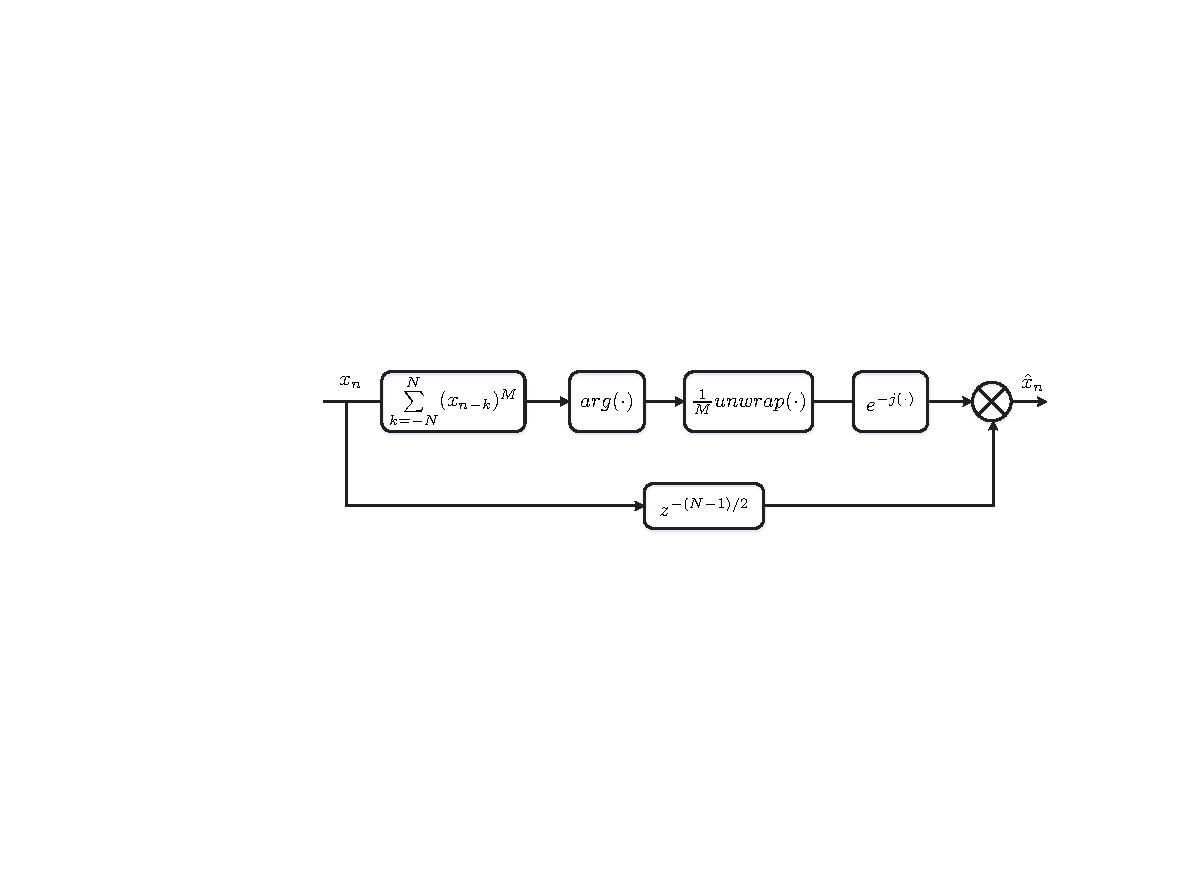
\includegraphics[width=\textwidth]{./sdf/dsp_laser_phase_compensation/figures/VV_phaseEstimation.pdf}
    \caption{Block diagram of Viterbi-Viterbi algorithm for carrier phase recovery.}
    \label{fig_VVdiagram}
\end{figure}
VV algorithm is a n-th power feed-forward approach employed for uniform angular distribution characteristic of m-PSK constellations, where the information of the modulated phase is removed by employing the n-th power operation on the received symbols. The algorithm implementation diagram is shown in Figure~\ref{fig_VVdiagram}, starting with M-th power operation on the received symbols. In order to minimize the impact of additive noise in the estimation process, a sum of $2N+1$ symbols is considered, which is then divided by M. The resulting estimated phase noise is then submitted to a phase unwrap function in order to avoid the occurrence of cycle slip. The final phase noise estimator is then used to compensate for the phase noise of the original symbol in the middle of the symbols block.


\subsubsection{Blind Phase Search Algorithm}
\begin{figure}[h!]
    \centering
    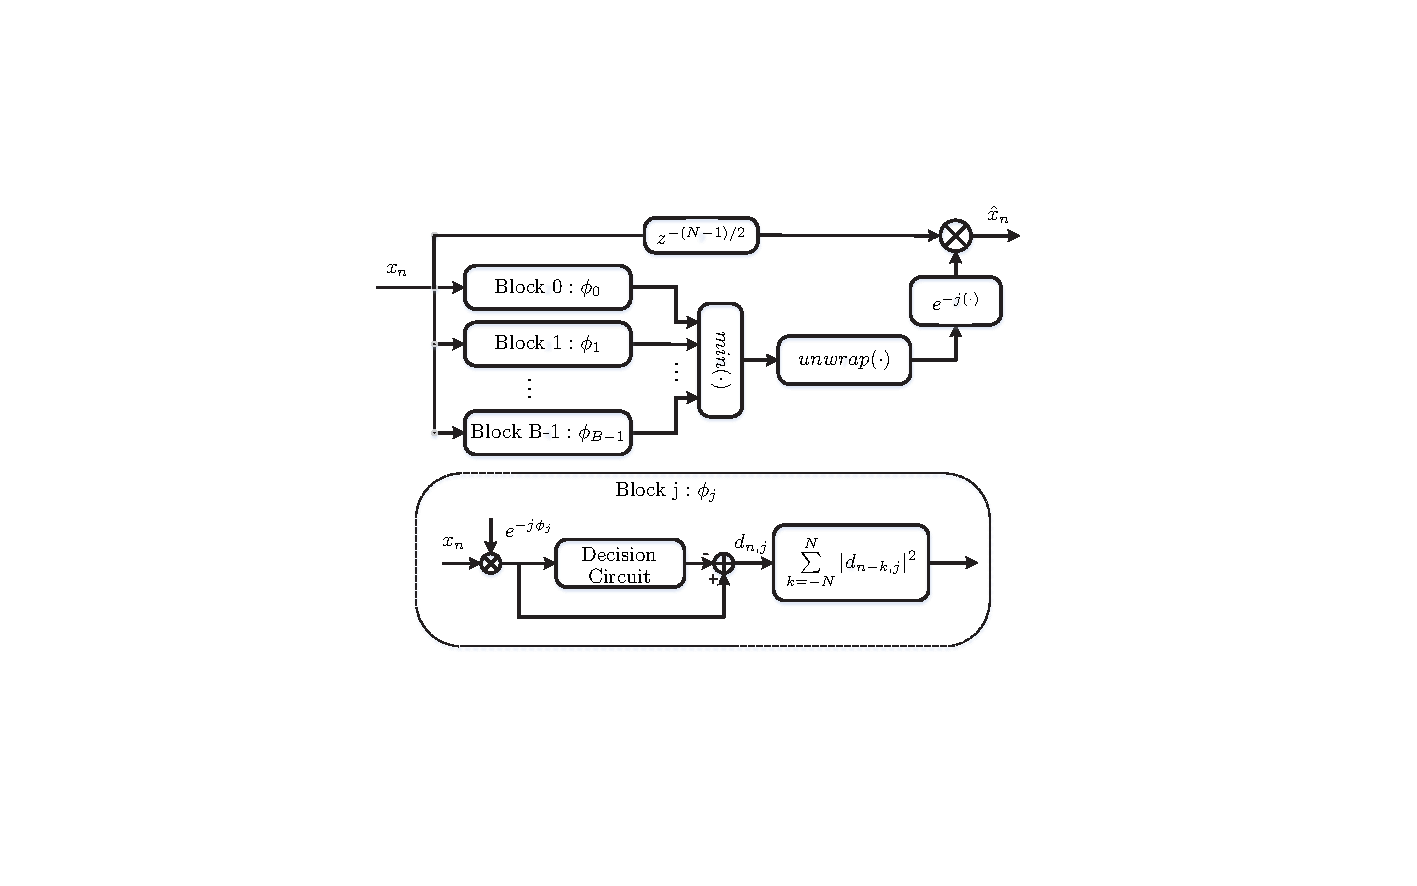
\includegraphics[width=12cm]{./sdf/dsp_laser_phase_compensation/figures/bps_diagram.pdf}
    \caption{Block diagram of blind phase search algorithm for carrier phase recovery.}
    \label{fig_BPSdiagram}
\end{figure}
An alternative to the VV phase noise estimator is the so-called BPS algorithm, in which the operation principle is shown in the Figure~\ref{fig_BPSdiagram}. Firstly, a block of $2N+1$ consecutive received symbols is rotated by a number of $B$ uniformly distributed test phases defined as,
\begin{equation}
    	\phi_{b} = \frac{b}{B}\frac{\pi}{2}, b \in\{0,1,...,B-1\}.
    \label{eq_phaseNoise}
\end{equation}
Then, the rotated blocks symbols are fed into decision circuit, where the square distance to the closest constellation points in the original constellation is calculated for each block. Each resulting square distances block is summed up to minimize the noise distortion. After average filtering, the test phase providing the minimum sum of distances is considered to be the phase noise estimator for the symbol in the middle of the block. The estimated phase noise is then unwrapped to reduce cycle slip occurrence, which is then used employed for the compensation for the phase noise of the original symbols.

\subsection{Simulation Analysis}
\begin{figure}[h!]
    \centering
    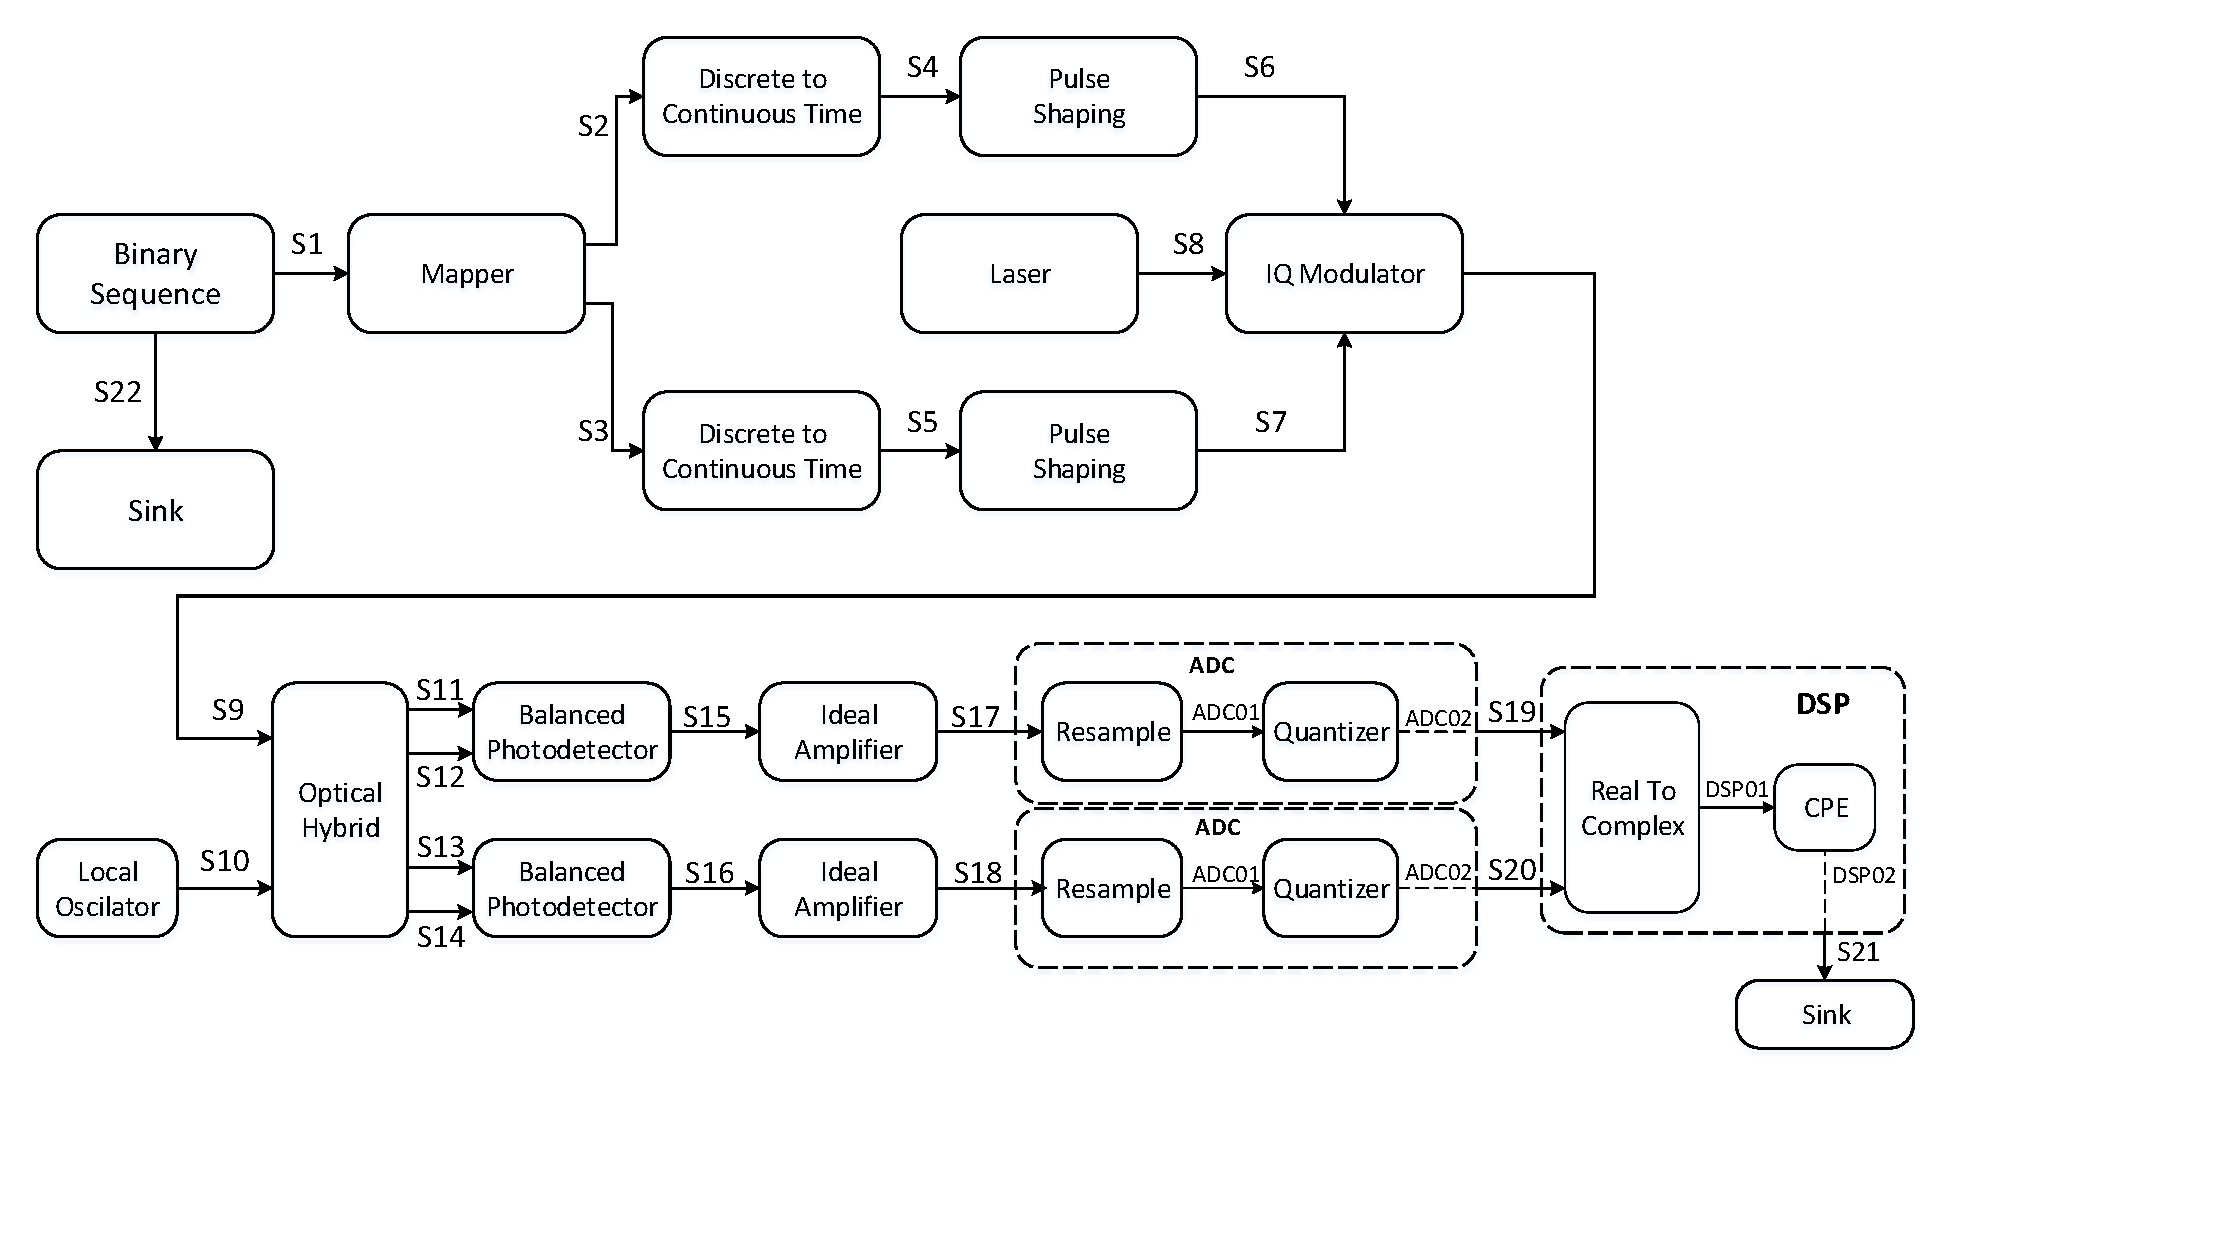
\includegraphics[width=15cm]{./sdf/dsp_laser_phase_compensation/figures/qpsk_transmitter_simulation.pdf}
    \caption{Simulation setup for the QPSK transmission system for the simulation of laser phase noise.}
    \label{fig_QPSKsystemLPN}
\end{figure}

Figure~\ref{fig_QPSKsystemLPN} depicts the simulation setup for a QPSK transmission system, including the simulation of carrier phase noise. As can be observed in the figure~\ref{fig_QPSKsystemLPN}, we have employed an IQ modulation which modulates the signal after pulse shaping, $S6$ and $S7$, on the laser carrier, $S8$. The output signal, $S9$, is then fed to coherent receiver front-end, comprising optical hybrid, photodiode and ideal amplifier. The output signal to the coherent receiver front-end, $S17$ and $S18$, are fed to the ADC super blocks, which comprises resample block followed by quantizer block. The two real output signals of ADC blocks, $S19$ and $S20$, are fed into DSP super block, where is performed the compensation of transmission impairments and recover of transmitted data. The DSP super block is composed in this case by a real to complex block, which combine the two input real signal into a complex signal and then fed to CPE block, where the laser phase noise compensation is performed. Then, the output, $S21$, is fed to the Sink block.

%\begin{table*}[h!]
    %\small
    \renewcommand{\arraystretch}{1.3}
    \centering
    \caption{System Input Parameters.}
    \label{system_input_parameters}%
    %\scalebox{0.85}{
    \resizebox{9cm}{!}{
    \begin{tabular}{|c|c|c|}
        \hline
        {$\text{Parameter}$}   & {$\text{Default Value}$}  &  {$\text{Description}$}  \\
        %\cline{2-3}
        \hline
        \hline
        {$\text{sourceMode}$}    & {}      &{}      \\
        \hline
        {$\text{patternLength}$}  & {}    &{}      \\
        \hline
        {$\text{numberOfBits}$}  & {}    &{}      \\
        \hline
        {$\text{bitPeriod}$}  & {}    &{}      \\
        \hline
        {$\text{iqAmplitudes}$}  & {}    &{}      \\
        \hline
        {$\text{samplePeriod}$}  & {}    &{}      \\
        \hline
        {$\text{numberOfSamplesPerSymbol}$}  & {}    &{}      \\
        \hline
        {$\text{filterType}$}  & {}    &{}      \\
        \hline
        {$\text{impulseResponseTimeLength}$}  & {}    &{}      \\
        \hline
        {$\text{rollOffFactor}$}  & {}    &{}      \\
        \hline
        {$\text{outputOpticalPower}$}  & {}    &{}      \\
        \hline
        {$\text{laserLW}$}  & {}    &{}      \\
        \hline
        {$\text{laserRIN}$}  & {}    &{}      \\
        \hline
    \end{tabular}}
\end{table*} 
%\begin{table*}[h!]
    \tiny
    \renewcommand{\arraystretch}{1.0}
    \centering
    \caption{Header Files for DSP Laser Phase Compensation.}
    \label{header_files}%
    %\scalebox{0.85}{
    \resizebox{9cm}{!}{
    \begin{tabular}{|c|c|c|}
        \hline
        {$\text{File Name}$}   & {$\text{Description}$}  &  {$\text{Status}$}  \\
        \hline
        \hline
        {$\text{binary_source.h}$}     &{}      &{\checkmark}      \\
        \hline
        {$\text{m\_qam\_mapper.h}$}     &{}      &{\checkmark}      \\
        \hline
        {$\text{discrete\_to\_continuous\_time.h}$}     &{}      &{\checkmark}      \\
        \hline
        {$\text{pulse\_shaper.h}$}  & {}    &{\checkmark}      \\
        \hline
        {$\text{local\_oscillator.h}$}  & {}    &{\checkmark}      \\
        \hline
        {$\text{iq\_modulator.h}$}  & {}    &{\checkmark}      \\
        \hline
        {$\text{sink.h}$}  & {}    &{\checkmark}      \\
        \hline
        {$\text{netxpto.h}$}  & {}    &{\checkmark}      \\
        \hline
    \end{tabular}}
\end{table*} 
%\begin{table*}[h!]
    \tiny
    \renewcommand{\arraystretch}{1.0}
    \centering
    \caption{Source Files for DSP Laser Phase Compensation.}
    \label{header_files}%
    %\scalebox{0.85}{
    \resizebox{9cm}{!}{
    \begin{tabular}{|c|c|c|}
        \hline
        {$\text{File Name}$}   & {$\text{Description}$}  &  {$\text{Status}$}  \\
        \hline
        \hline
        {$\text{binary_source.cpp}$}     &{}      &{\checkmark}      \\
        \hline
        {$\text{m\_qam\_mapper.cpp}$}     &{}      &{\checkmark}      \\
        \hline
        {$\text{discrete\_to\_continuous\_time.cpp}$}     &{}      &{\checkmark}      \\
        \hline
        {$\text{pulse\_shaper.cpp}$}  & {}    &{\checkmark}      \\
        \hline
        {$\text{local\_oscillator.cpp}$}  & {}    &{\checkmark}      \\
        \hline
        {$\text{iq\_modulator.cpp}$}  & {}    &{\checkmark}      \\
        \hline
        {$\text{sink.cpp}$}  & {}    &{\checkmark}      \\
        \hline
        {$\text{netxpto.cpp}$}  & {}    &{\checkmark}      \\
        \hline
    \end{tabular}}
\end{table*} 

\subsection{Simulation Results}

The time-domain output signal of IQ modulator $S9$ is presented in figure~\ref{fig_s9} (a) and its corresponding constellation diagram is shown in figure~\ref{fig_s9} (b). From the figure~\ref{fig_s9} (b) it can be clearly observed the effect of laser phase noise, where the signal $S9$ presents a rotated constellation points. In general, the amount of the rotation is directly proportional to by the laser linewidth and the signal symbol rate.

\begin{figure}[h!]
\centering
\begin{subfigure}{.5\textwidth}
  \centering
  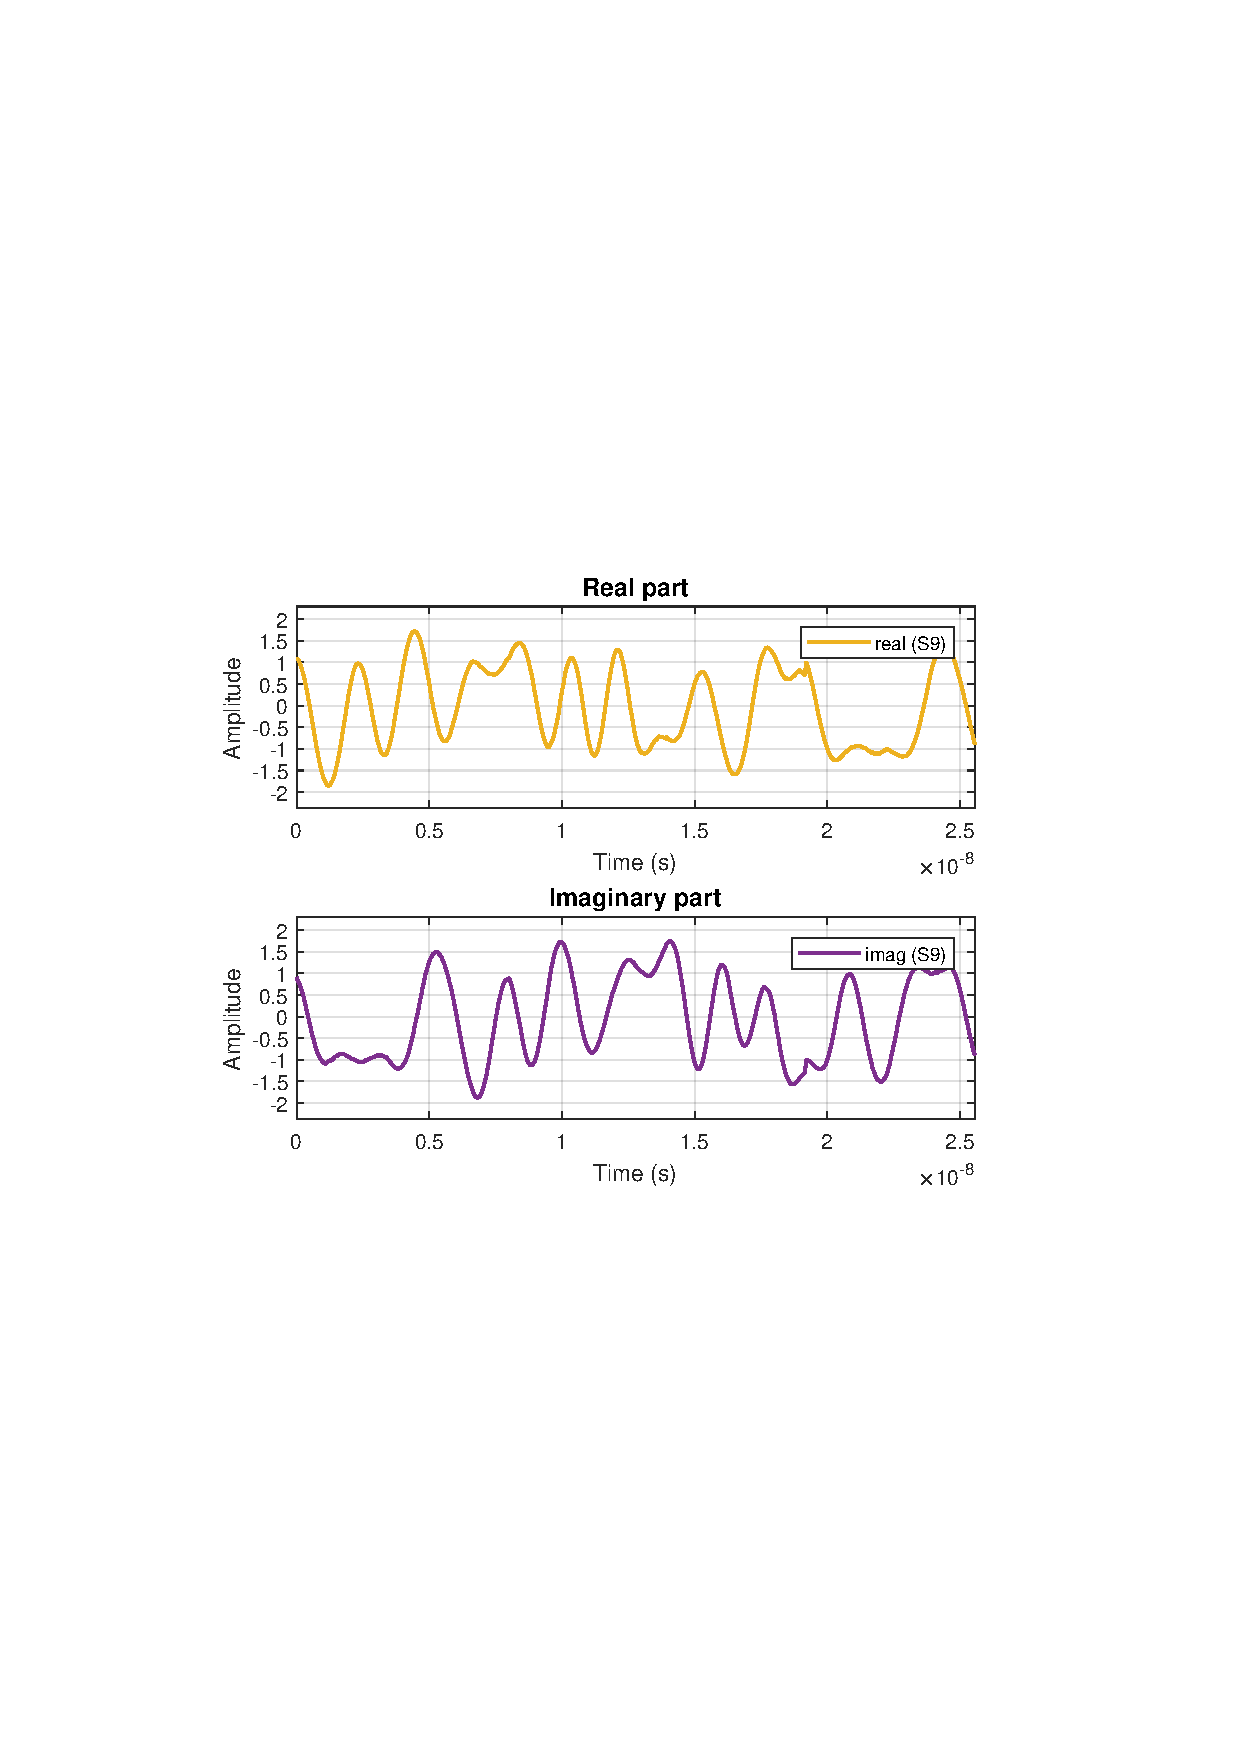
\includegraphics[width=\linewidth]{./sdf/dsp_laser_phase_compensation/figures/S9_td.pdf}
  \caption{}
  \label{fig:sub1}
\end{subfigure}%
\begin{subfigure}{.5\textwidth}
  \centering
  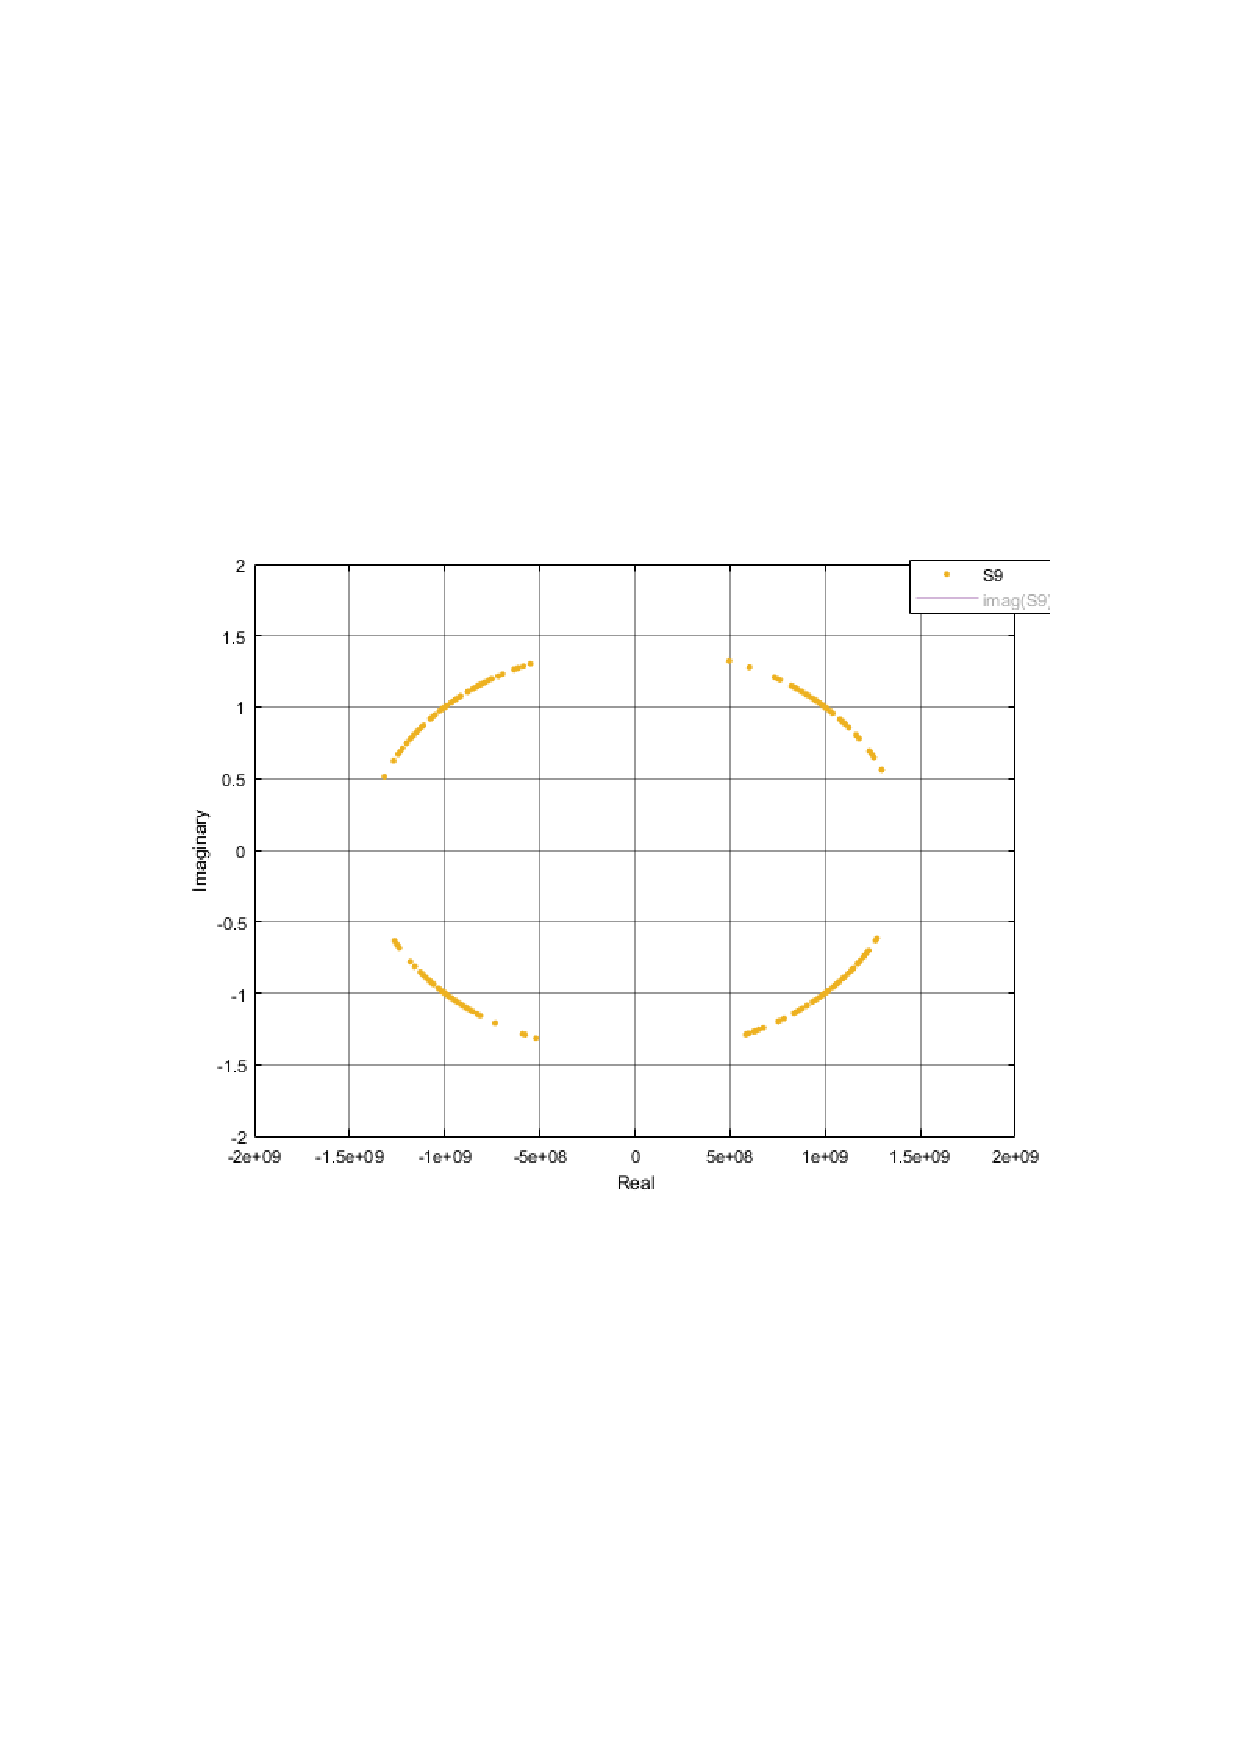
\includegraphics[width=\linewidth]{./sdf/dsp_laser_phase_compensation/figures/S9_constl.pdf}
  \caption{}
  \label{fig:sub2}
\end{subfigure}
\caption{Output sinal of IQ modulator, $S9$, including the laser phase noise. (a) Time-domain; (b) Constellations diagram.}
\label{fig_s9}
\end{figure}


\begin{figure}[h!]
\centering
\begin{subfigure}{.5\textwidth}
  \centering
  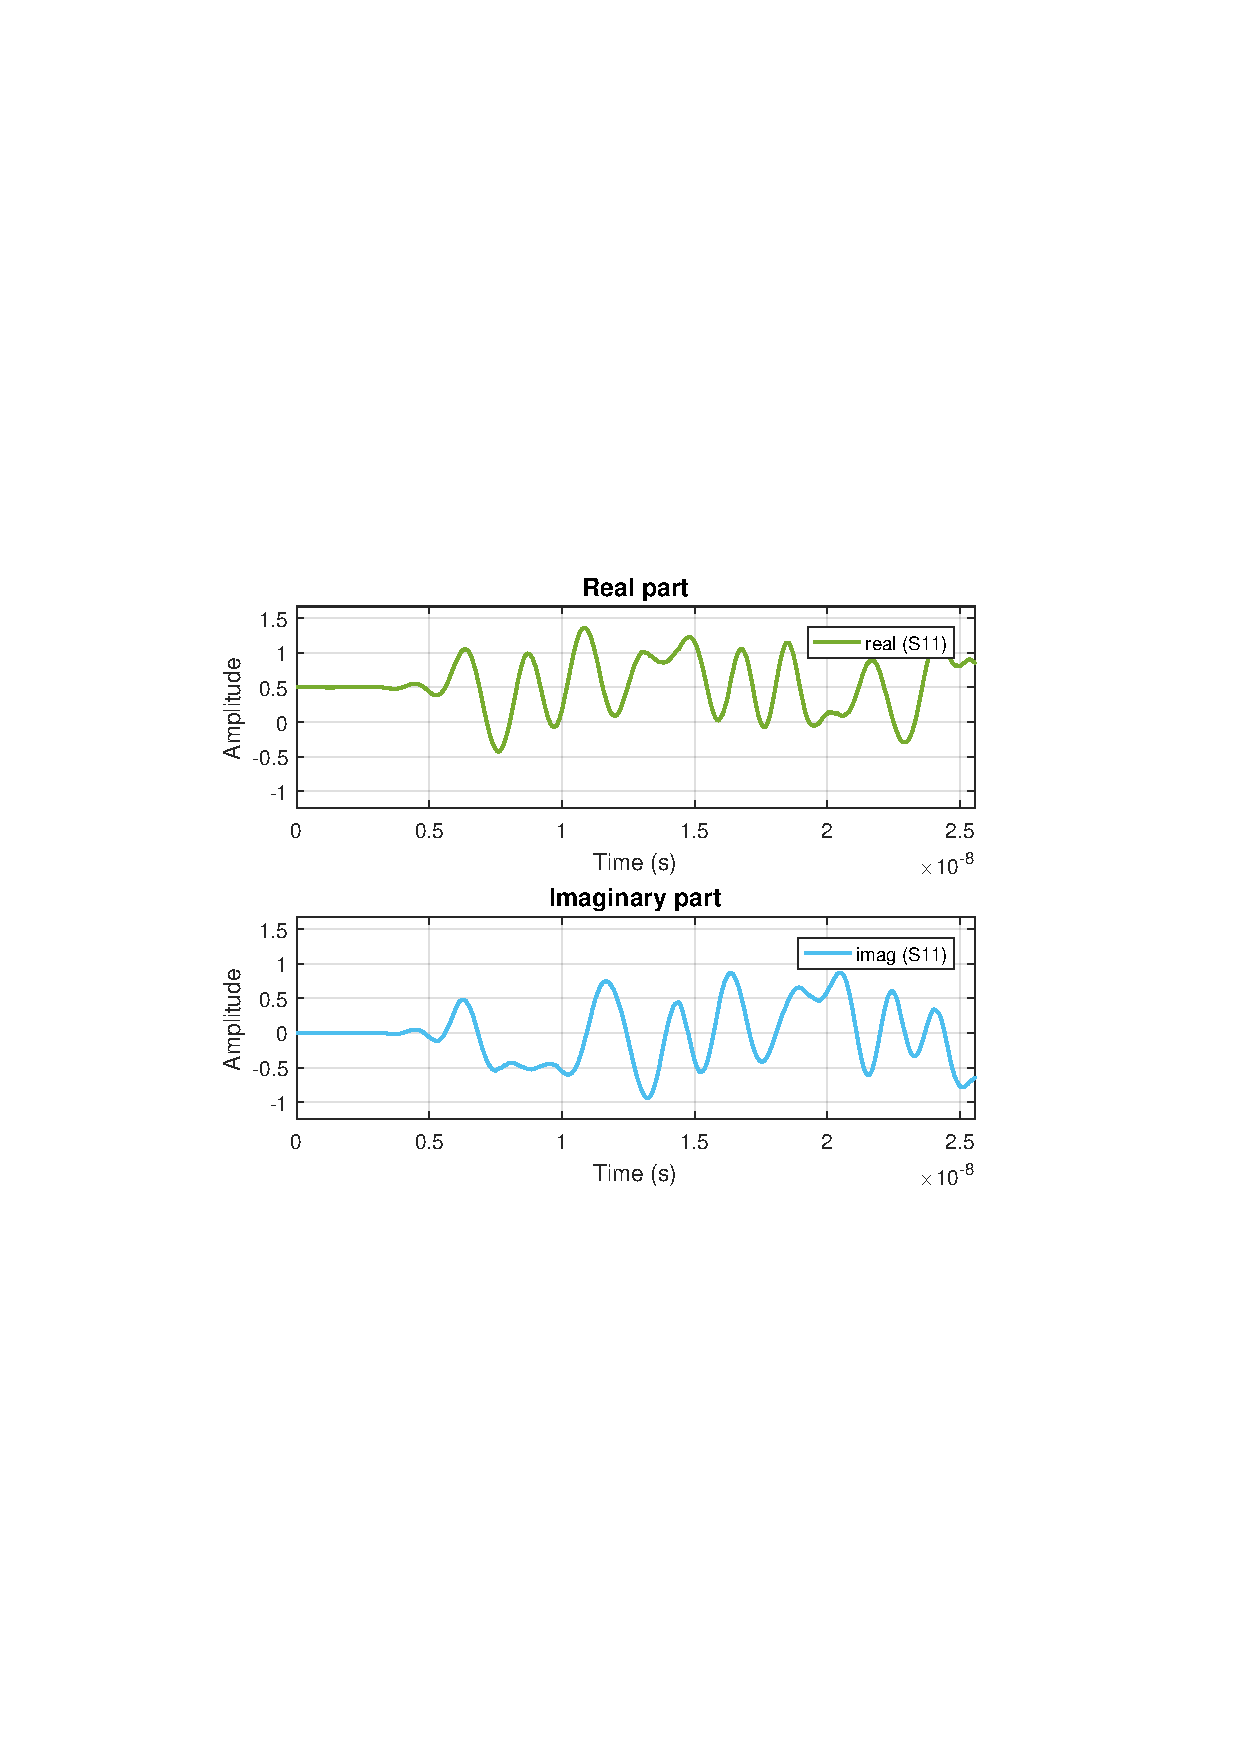
\includegraphics[width=\linewidth]{./sdf/dsp_laser_phase_compensation/figures/S11_td.pdf}
  \caption{}
  \label{fig:sub1}
\end{subfigure}%
\begin{subfigure}{.5\textwidth}
  \centering
  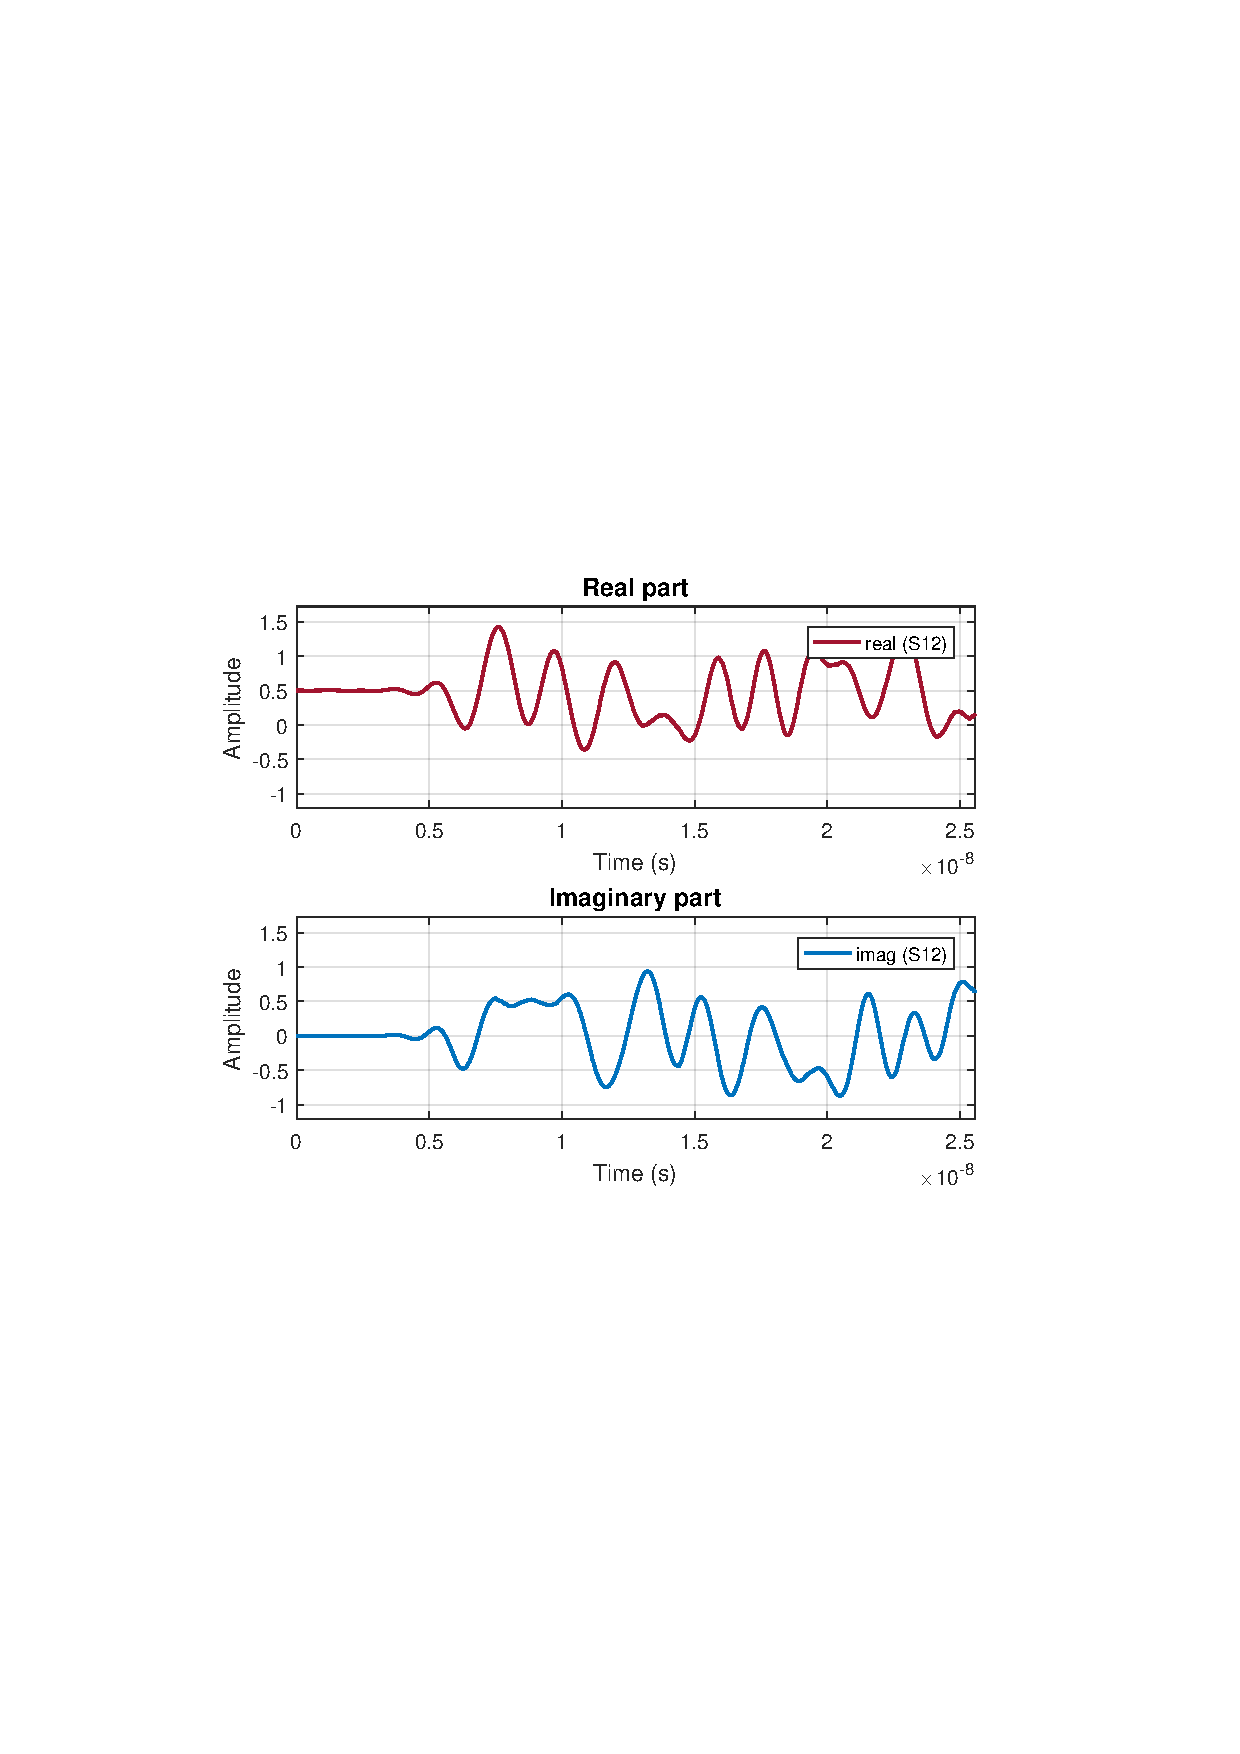
\includegraphics[width=\linewidth]{./sdf/dsp_laser_phase_compensation/figures/S12_td.pdf}
  \caption{}
  \label{fig:sub2}
\end{subfigure}
\caption{The in-phase output of optical hybrid block. (a) $S11$; (b) $S11$.}
\label{fig_s11_12}
\end{figure}


The in-phase and quadrature of signal are obtained by using the optical hybrid, which is illustrated in the figure~\ref{fig_s11_12} and figure~\ref{fig_s15_16}, respectively.

\begin{figure}[h!]
\centering
\begin{subfigure}{.5\textwidth}
  \centering
  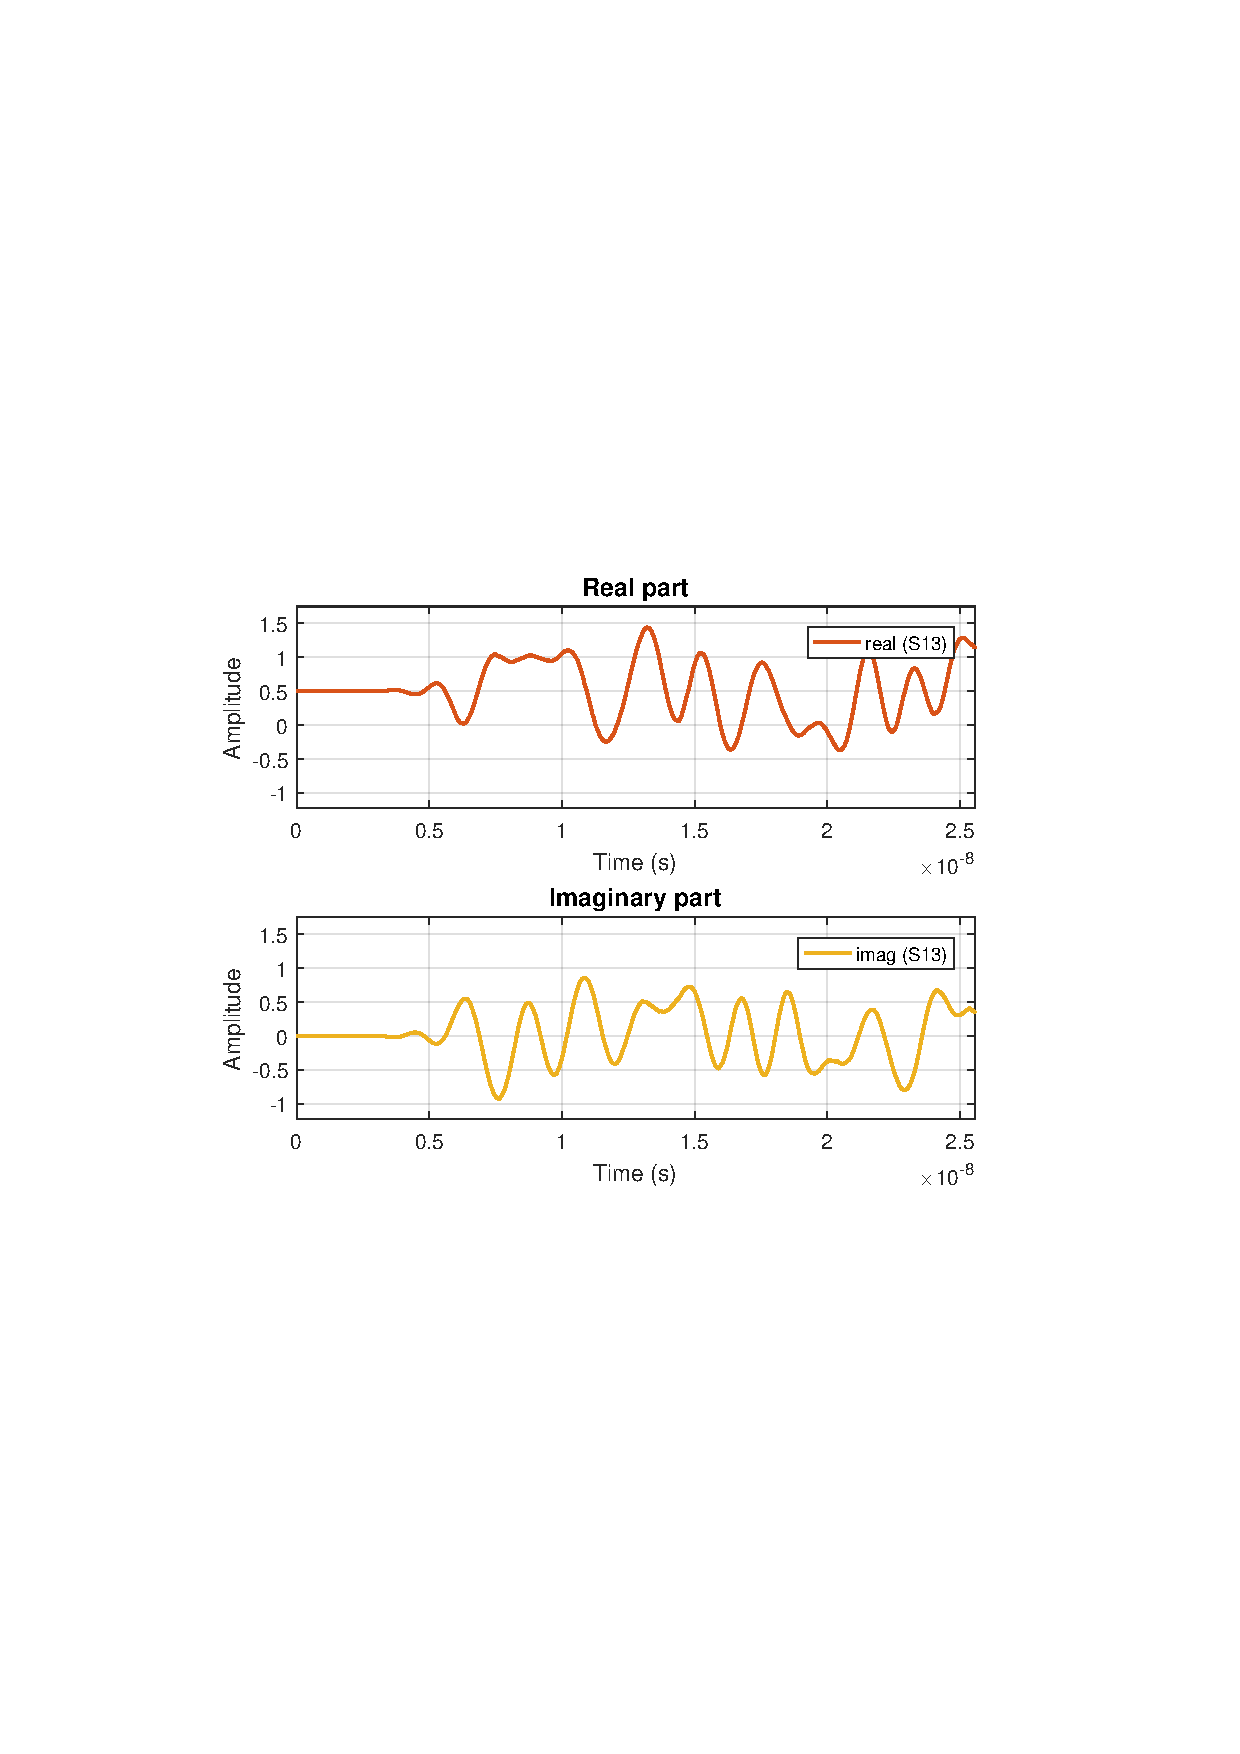
\includegraphics[width=\linewidth]{./sdf/dsp_laser_phase_compensation/figures/S13_td.pdf}
  \caption{}
  \label{fig:sub1}
\end{subfigure}%
\begin{subfigure}{.5\textwidth}
  \centering
  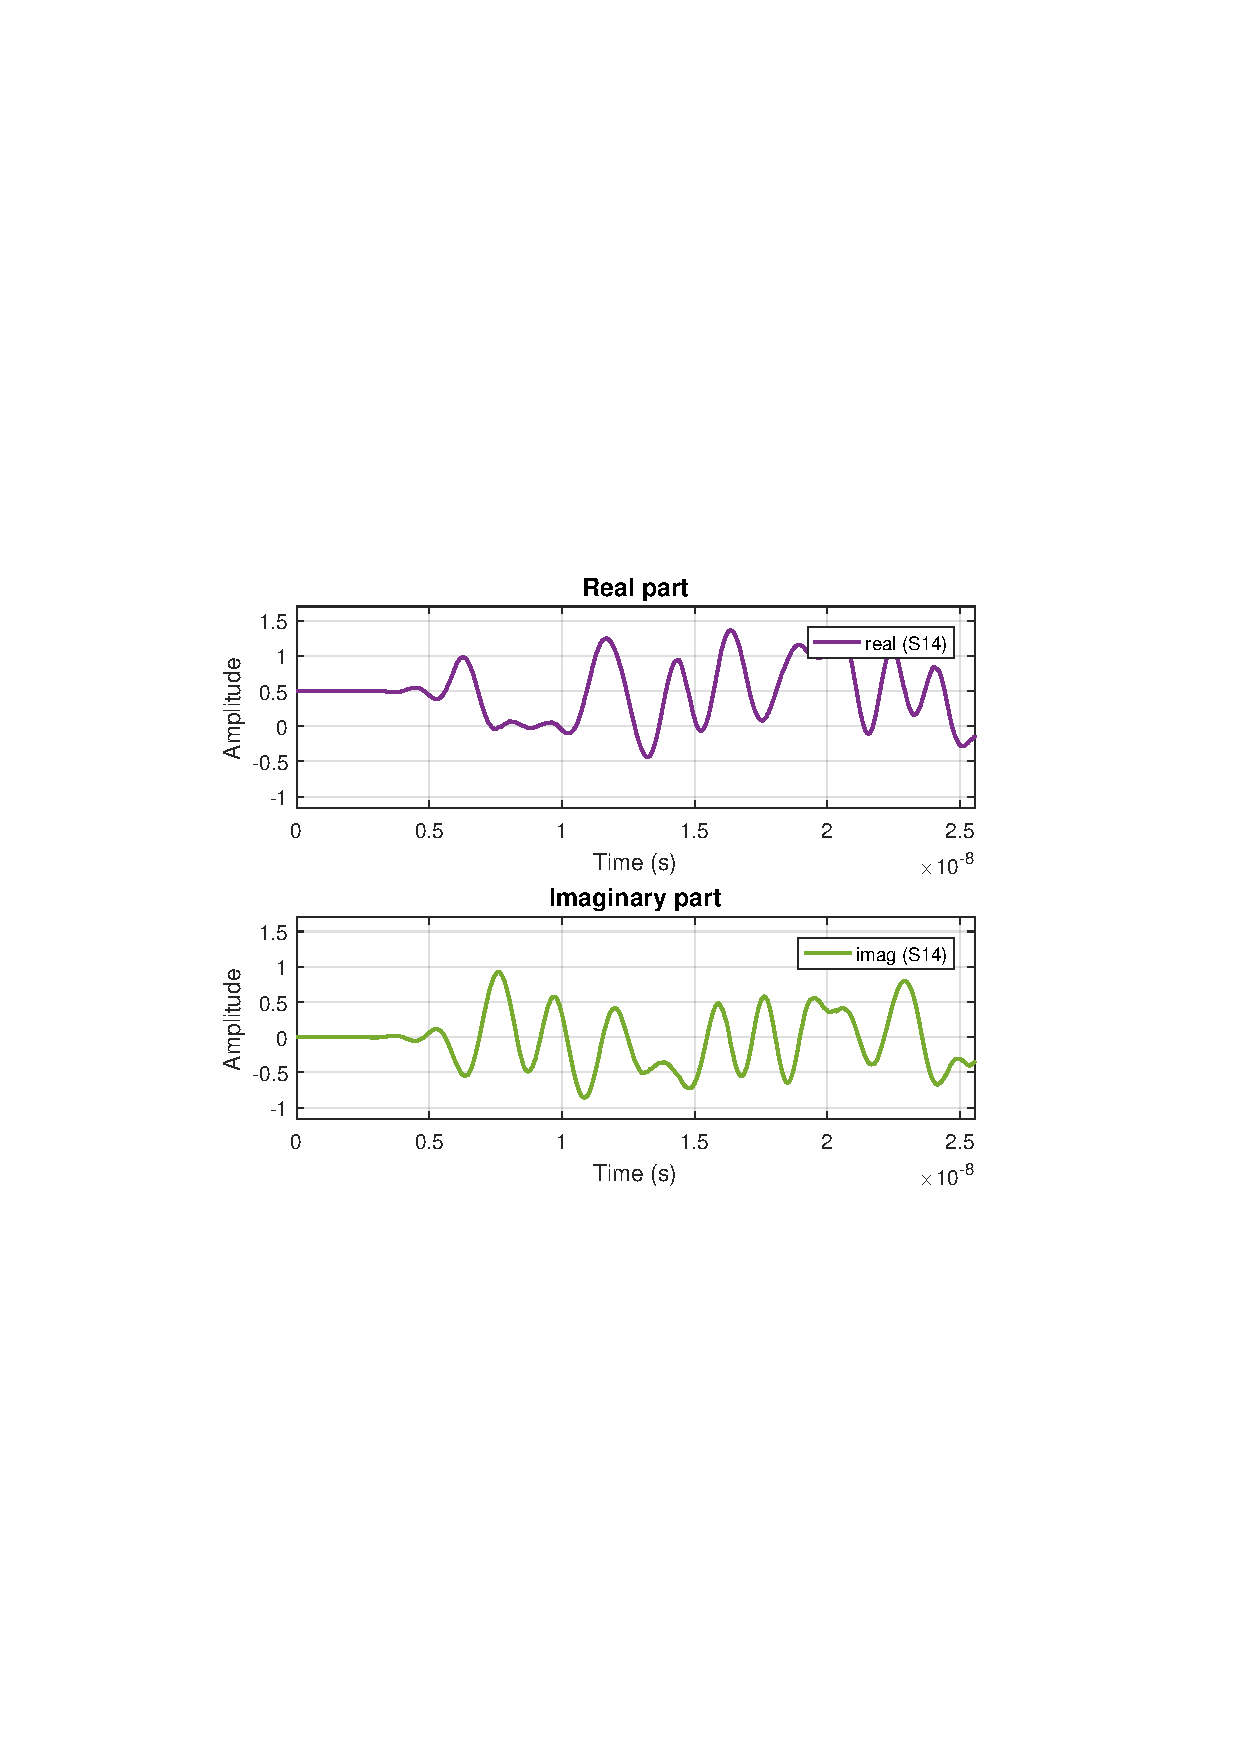
\includegraphics[width=\linewidth]{./sdf/dsp_laser_phase_compensation/figures/S14_td.pdf}
  \caption{}
  \label{fig:sub2}
\end{subfigure}
\caption{The quadrature output of optical hybrid block. (a) $S13$; (b) $S14$.}
\label{fig_s11_12}
\end{figure}

The signal after balanced photodiodes is presented in the figure~\ref{fig_s15_16}.

\begin{figure}[h!]
\centering
\begin{subfigure}{.5\textwidth}
  \centering
  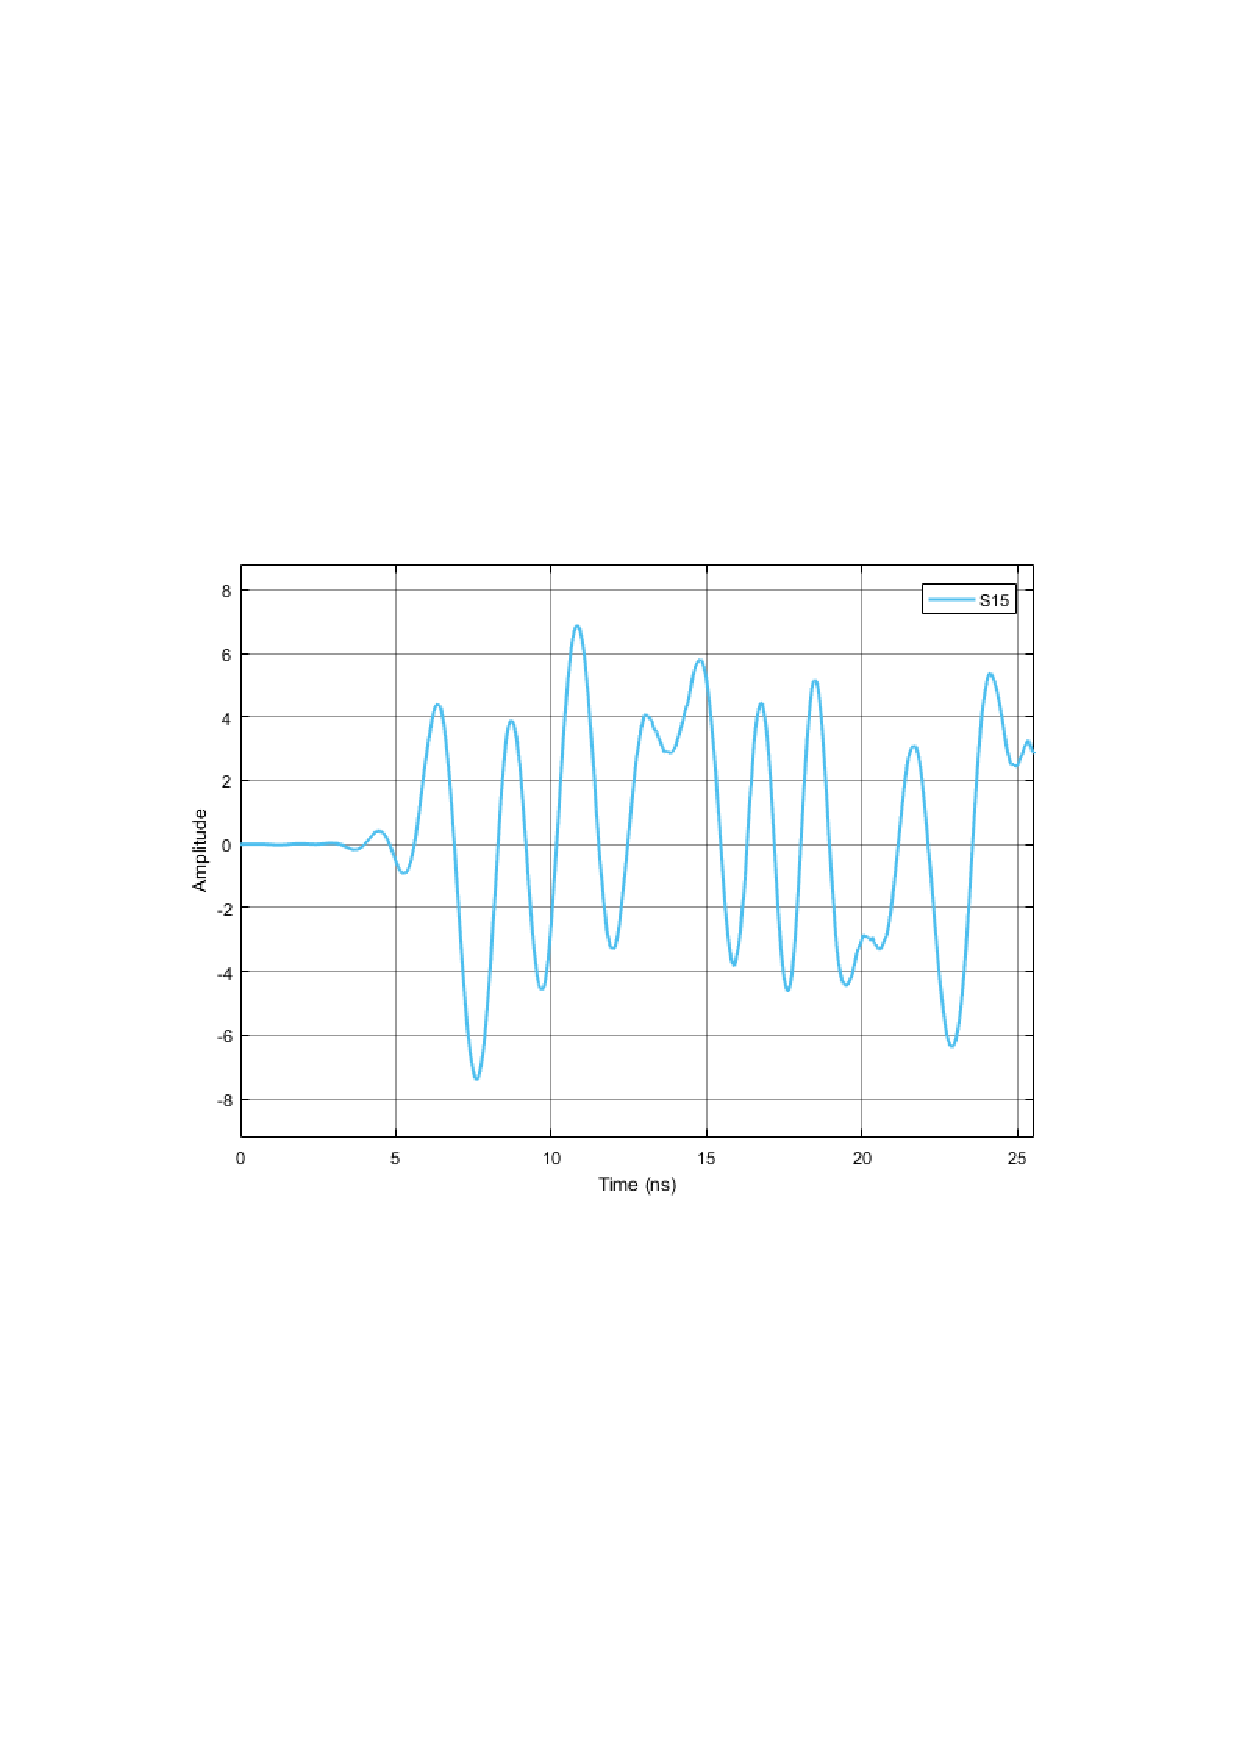
\includegraphics[width=\linewidth]{./sdf/dsp_laser_phase_compensation/figures/S15_td.pdf}
  \caption{}
  \label{fig:sub1}
\end{subfigure}%
\begin{subfigure}{.5\textwidth}
  \centering
  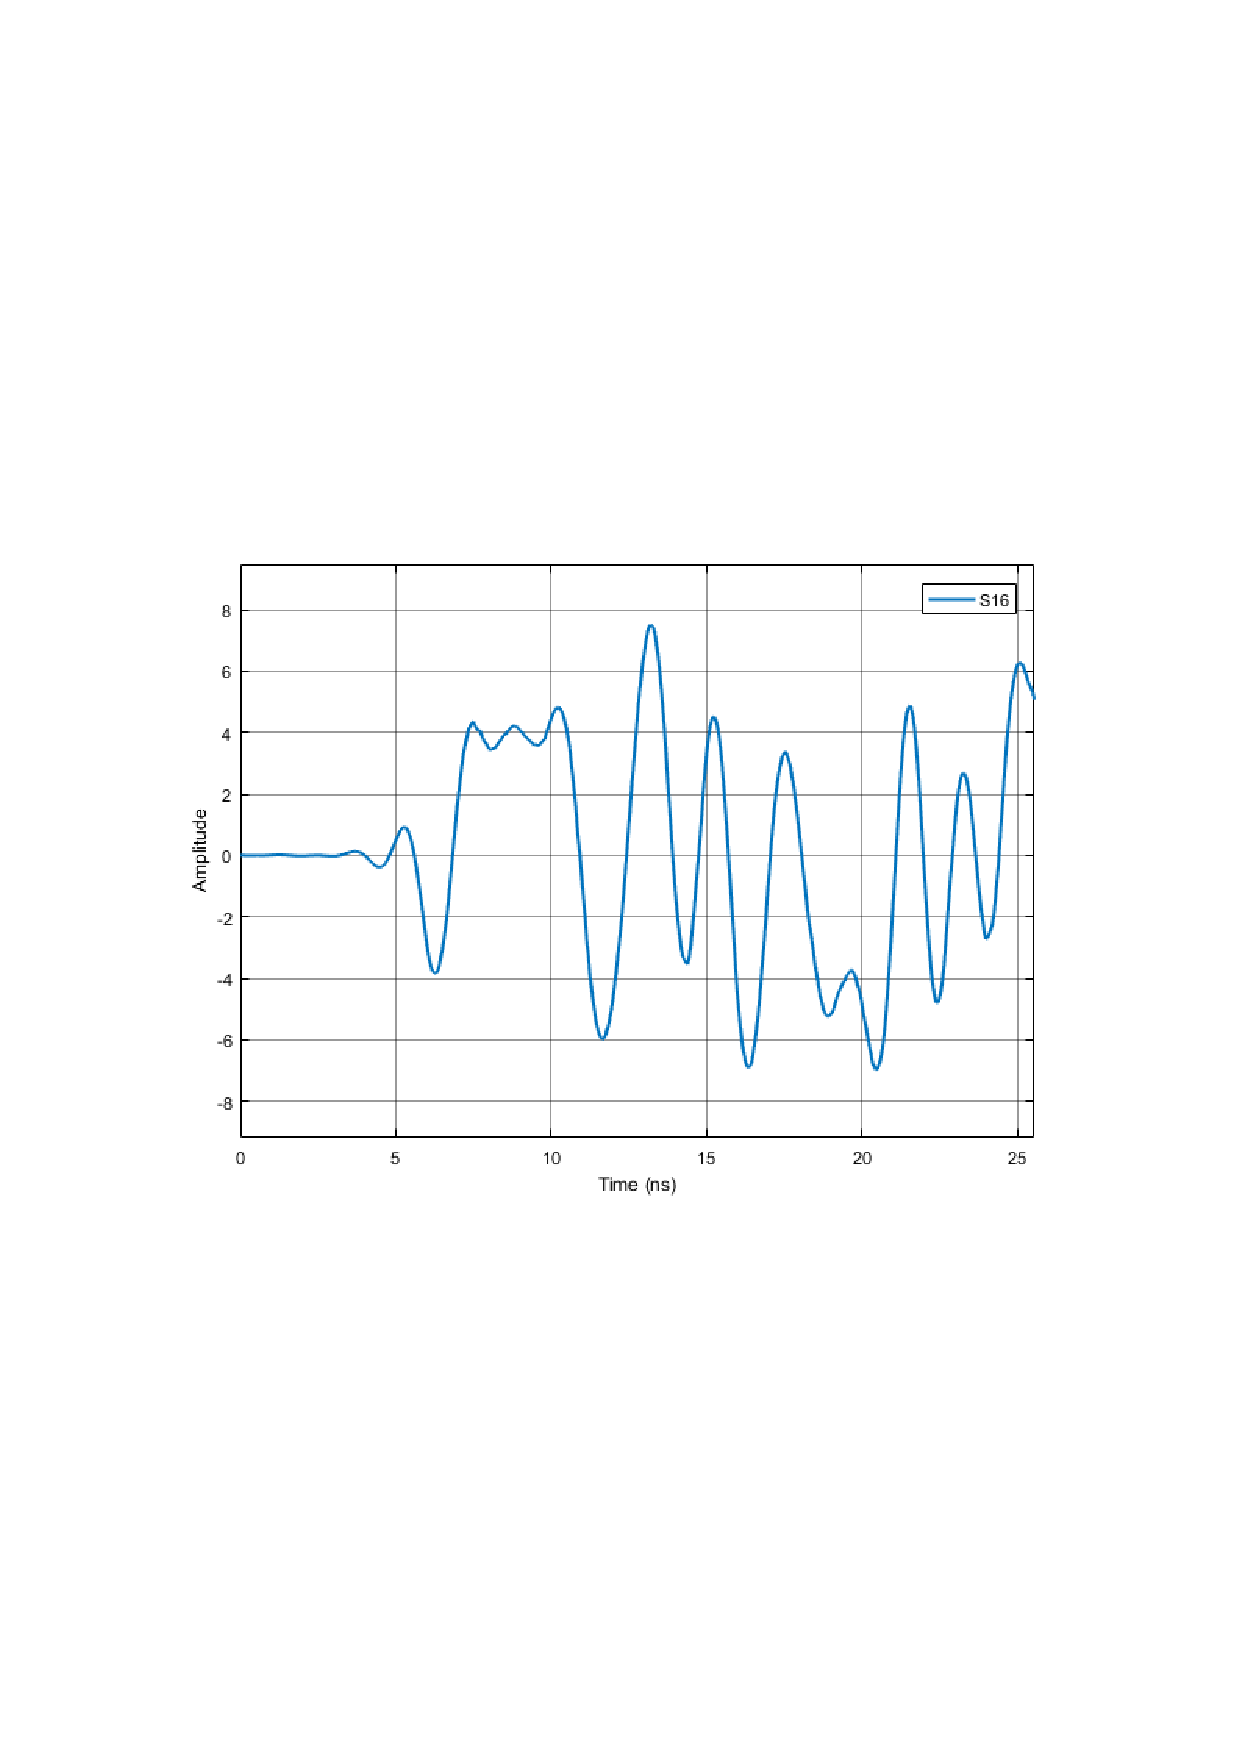
\includegraphics[width=\linewidth]{./sdf/dsp_laser_phase_compensation/figures/S16_td.pdf}
  \caption{}
  \label{fig:sub2}
\end{subfigure}
\caption{The output signal of balanced photodiodes block. (a) In-phase component, $S15$; (b)  Quadrature component, $S16$.}
\label{fig_s15_16}
\end{figure}

\pagebreak

The signal at the output of the amplifier is shown in the figure~\ref{fig_s17_18}.

\begin{figure}[h!]
\centering
\begin{subfigure}{.5\textwidth}
  \centering
  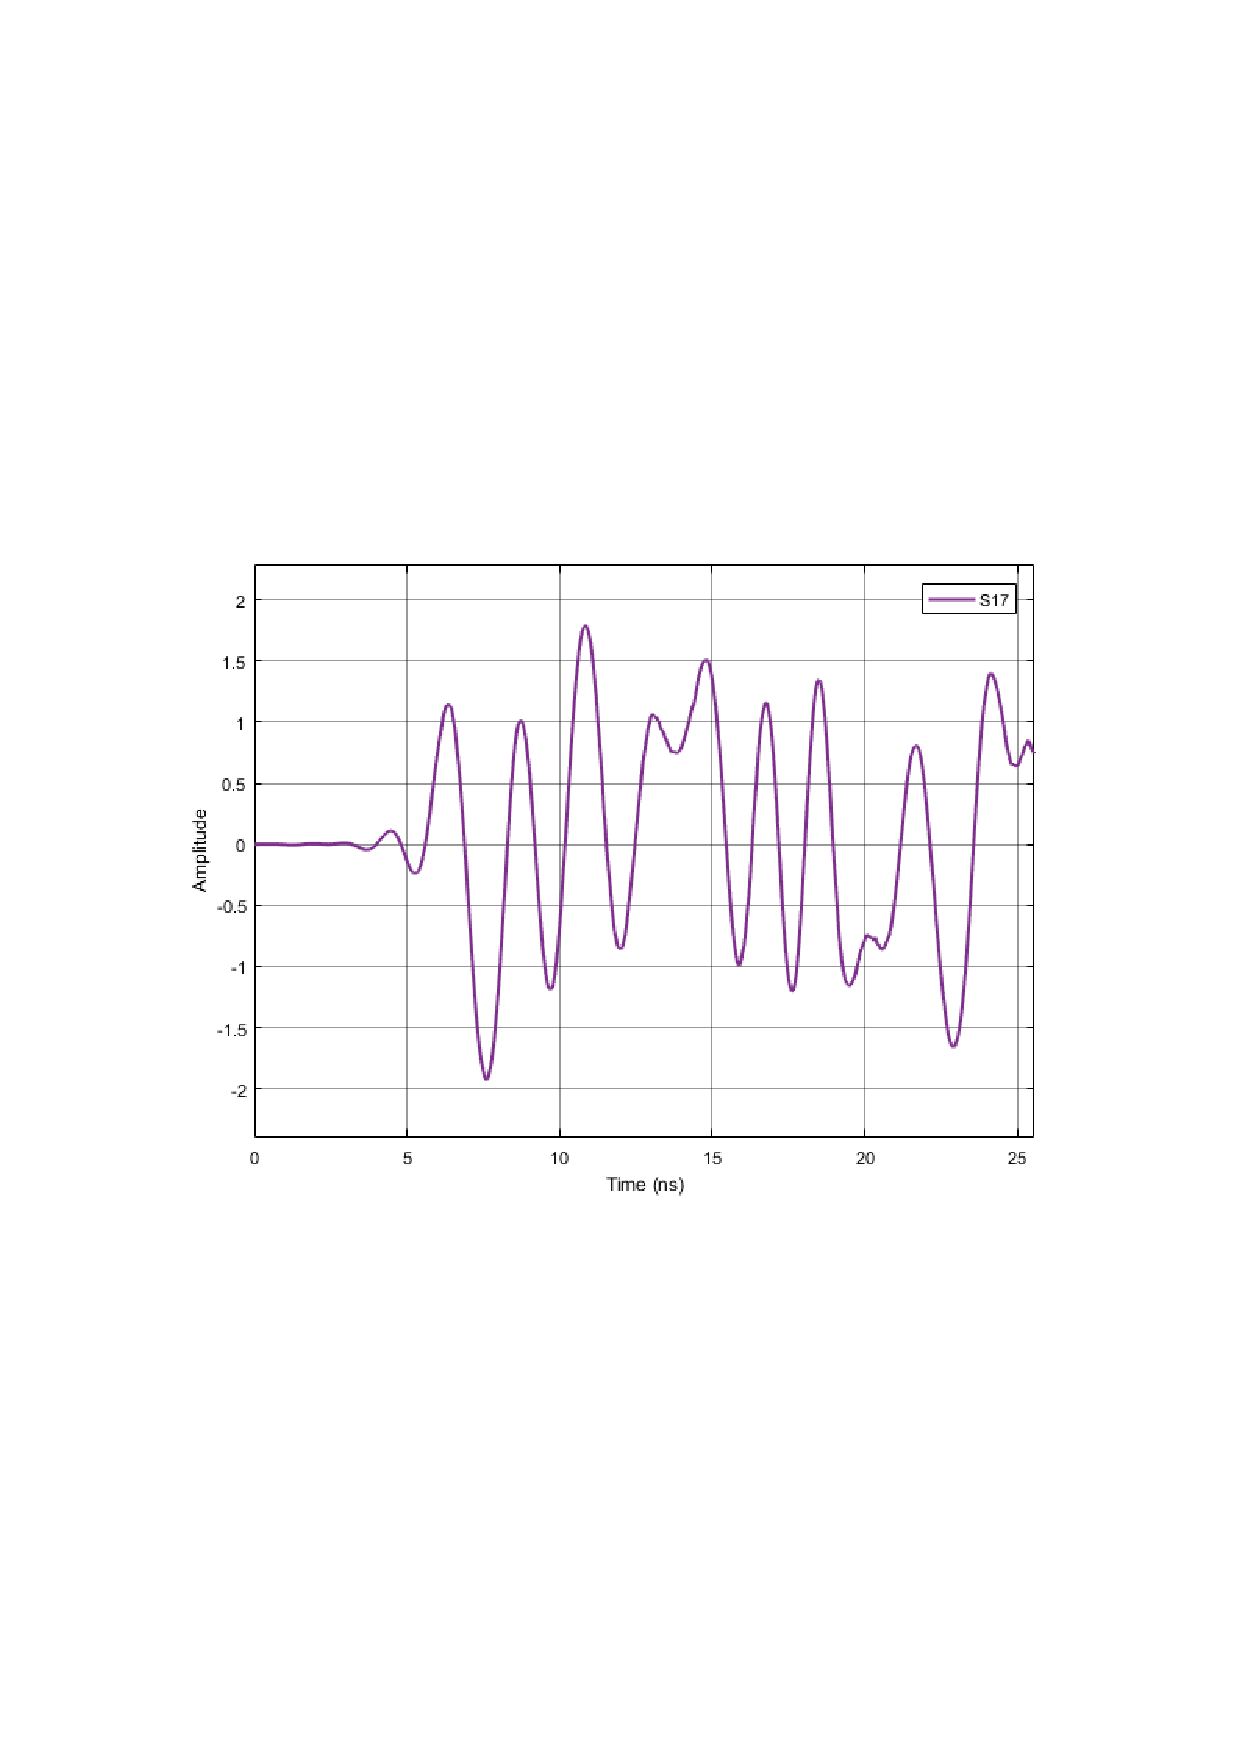
\includegraphics[width=\linewidth]{./sdf/dsp_laser_phase_compensation/figures/S17_td.pdf}
  \caption{}
  \label{fig:sub1}
\end{subfigure}%
\begin{subfigure}{.5\textwidth}
  \centering
  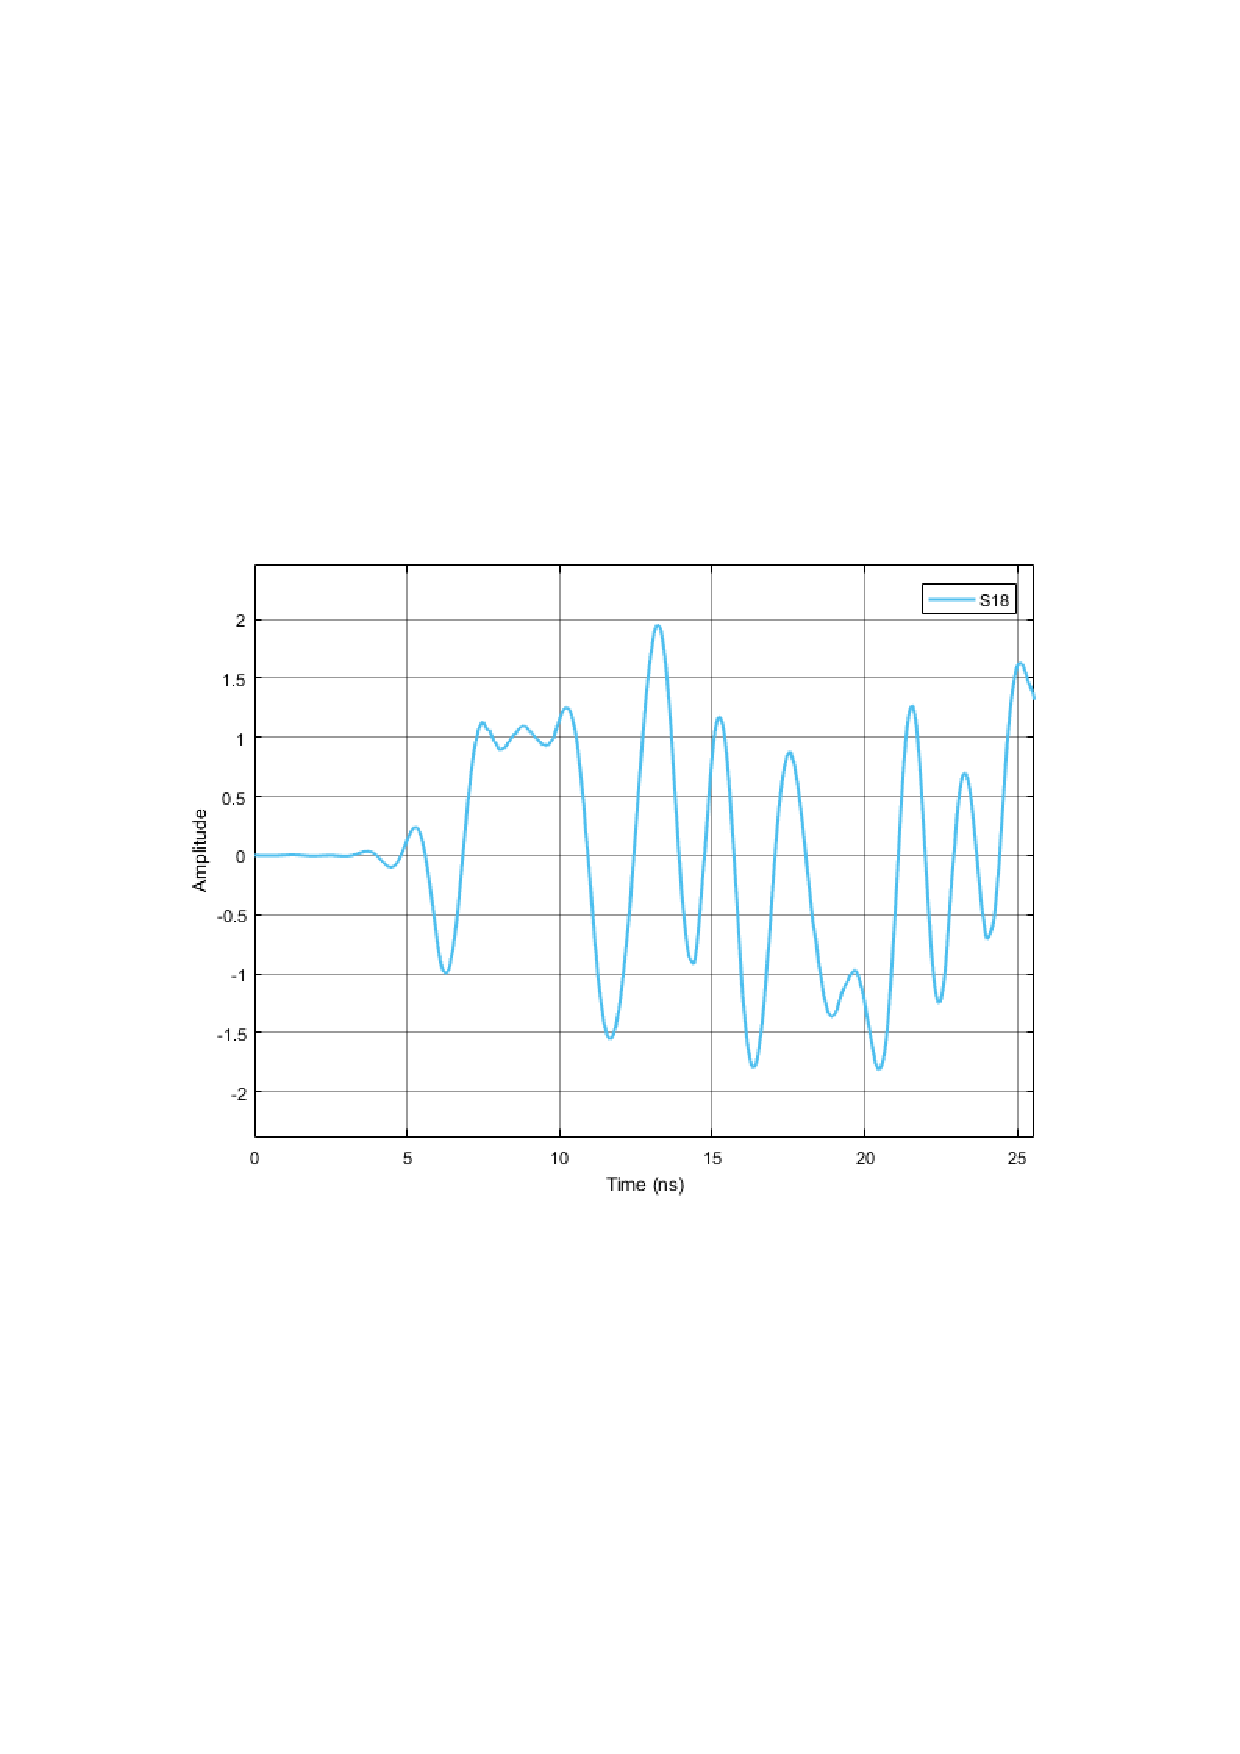
\includegraphics[width=\linewidth]{./sdf/dsp_laser_phase_compensation/figures/S18_td.pdf}
  \caption{}
  \label{fig:sub2}
\end{subfigure}
\caption{The output signal of the ideal amplifier block. (a) In-phase component, $S17$; (b)  Quadrature component, $S18$.}
\label{fig_s17_18}
\end{figure}


The signal after the super block ADC is shown in the figure~\ref{fig_s21}


\begin{figure}[h!]
\centering
\begin{subfigure}{.5\textwidth}
  \centering
  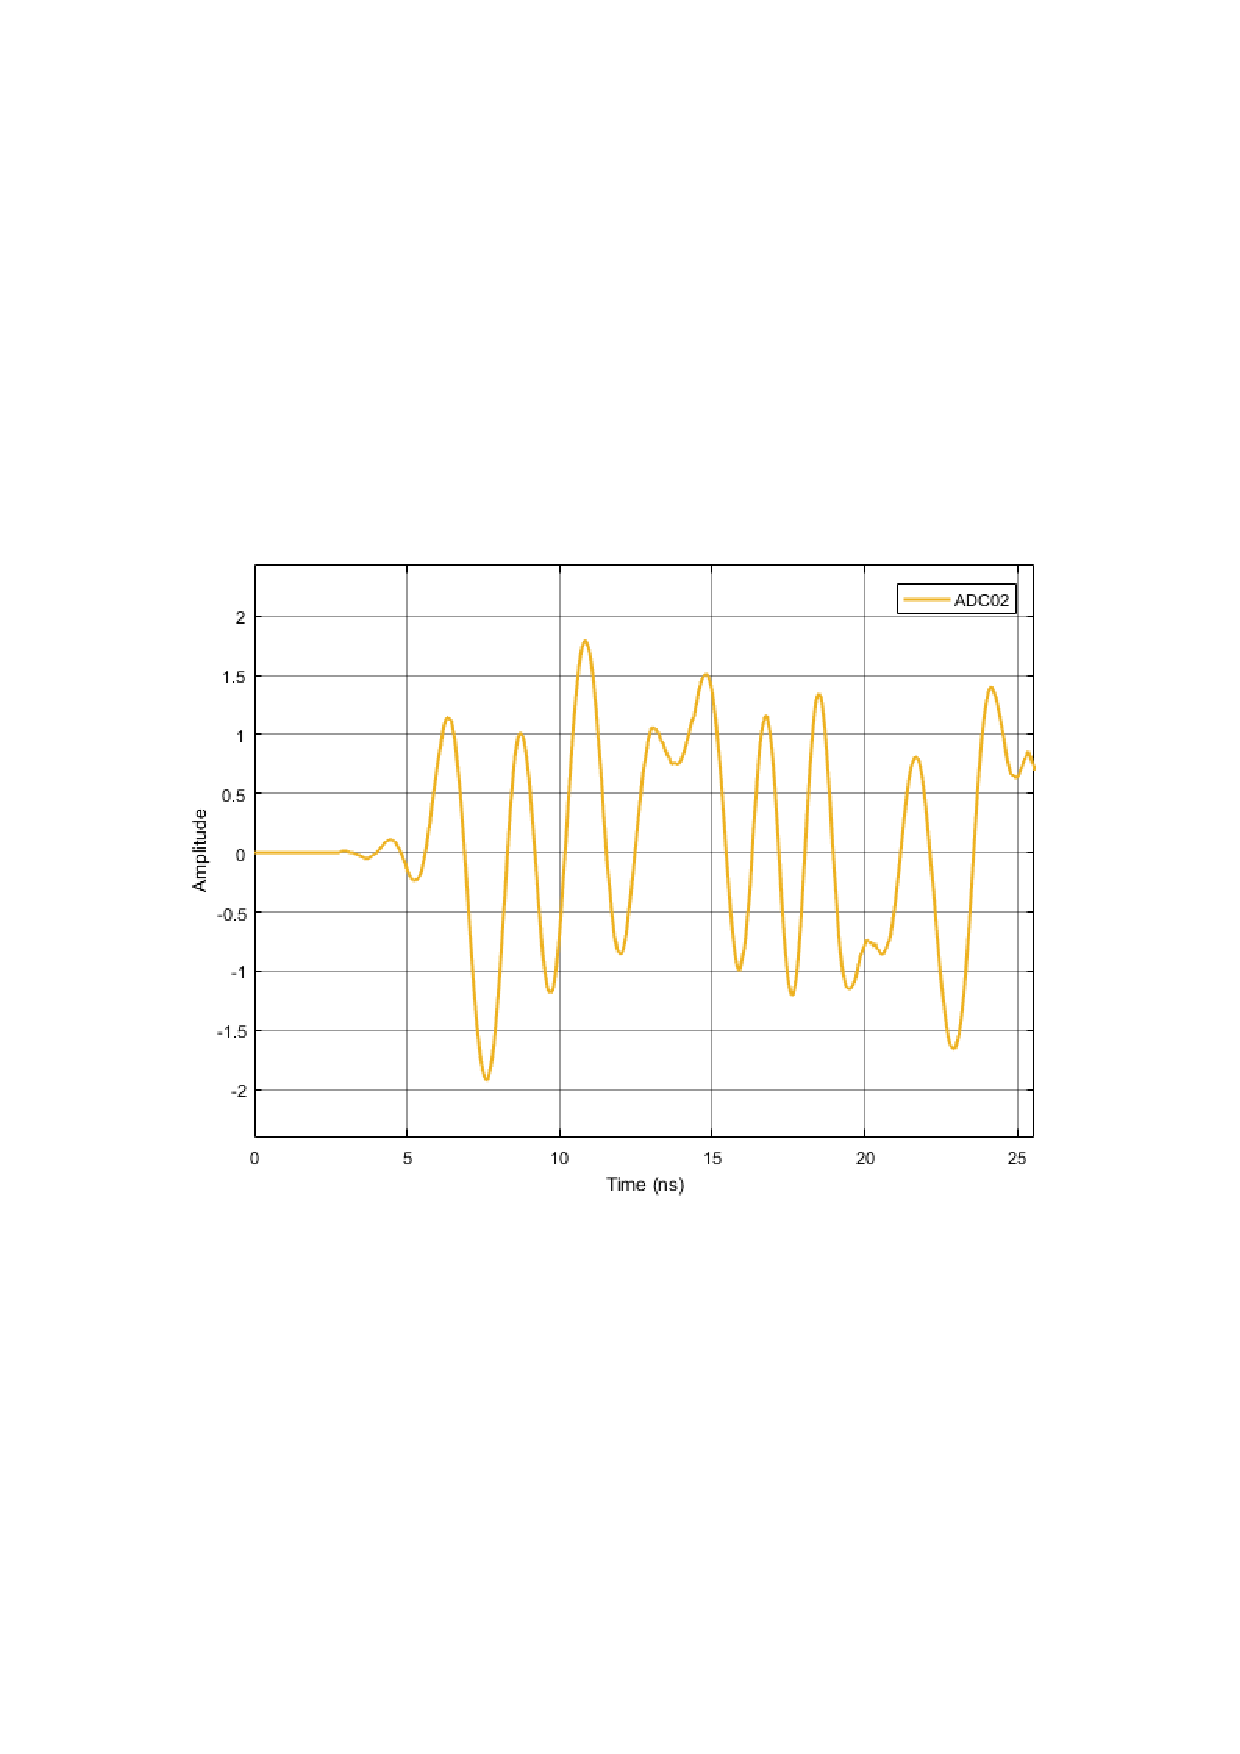
\includegraphics[width=\linewidth]{./sdf/dsp_laser_phase_compensation/figures/S21_td_8bits.pdf}
  \caption{}
  \label{fig:sub1}
\end{subfigure}%
\begin{subfigure}{.5\textwidth}
  \centering
  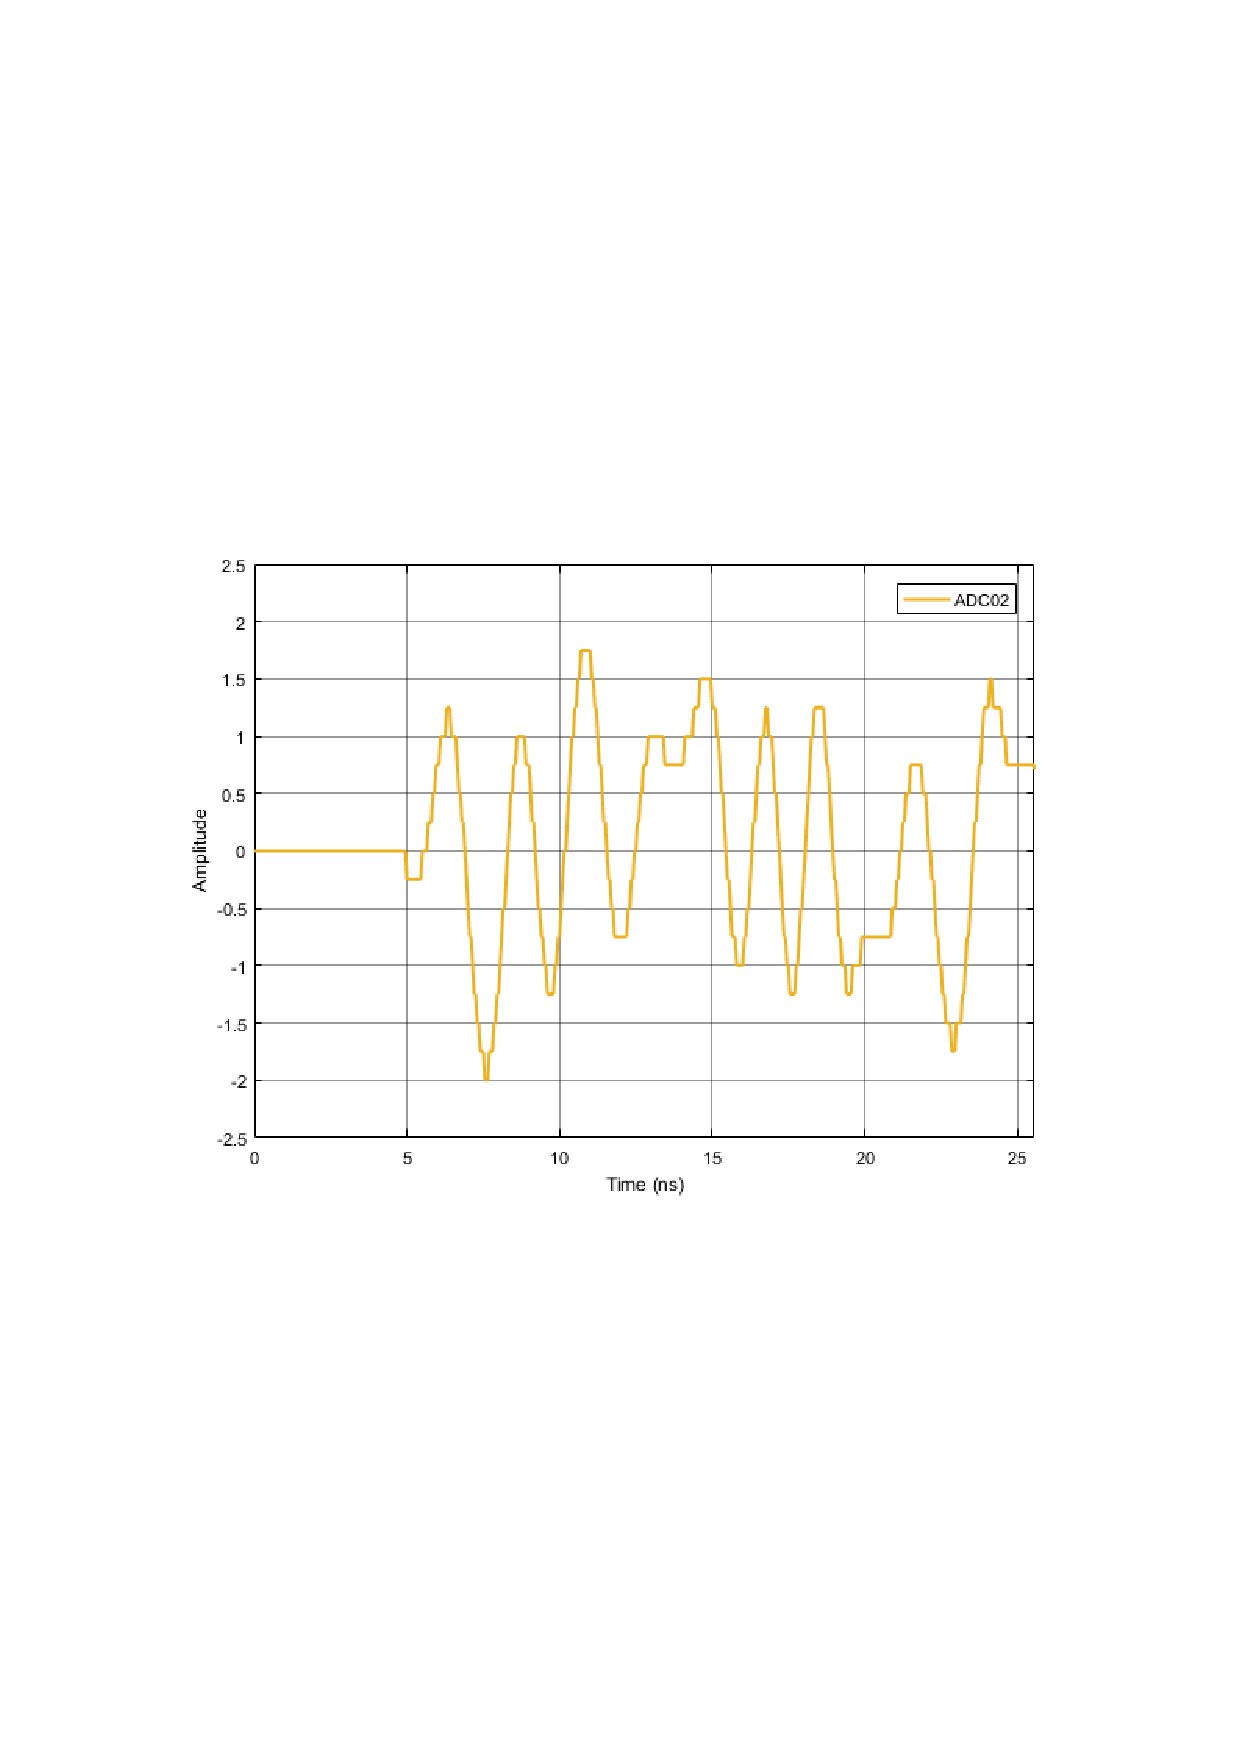
\includegraphics[width=\linewidth]{./sdf/dsp_laser_phase_compensation/figures/S21_td_4bits.pdf}
  \caption{}
  \label{fig:sub2}
\end{subfigure}
\caption{The output signal of the ADC super block, which includes the resample and quantizer blocks. (a) 8-bits quantization signal; (b)  4-bits quantization signal.}
\label{fig_s21}
\end{figure}

\pagebreak

Figure~\ref{fig_s24} and Figure~\ref{fig_s24_bps} show the signal after phase noise compensation using VV and BPS algorithms, respectively. As we can note in the figure~\ref{fig_s24} (b) and figure~\ref{fig_s24_bps} (b), the correct constellation diagram points is recovered, which indicates that the laser phase noise is effectively compensated.

\begin{figure}[h!]
\centering
\begin{subfigure}{.5\textwidth}
  \centering
  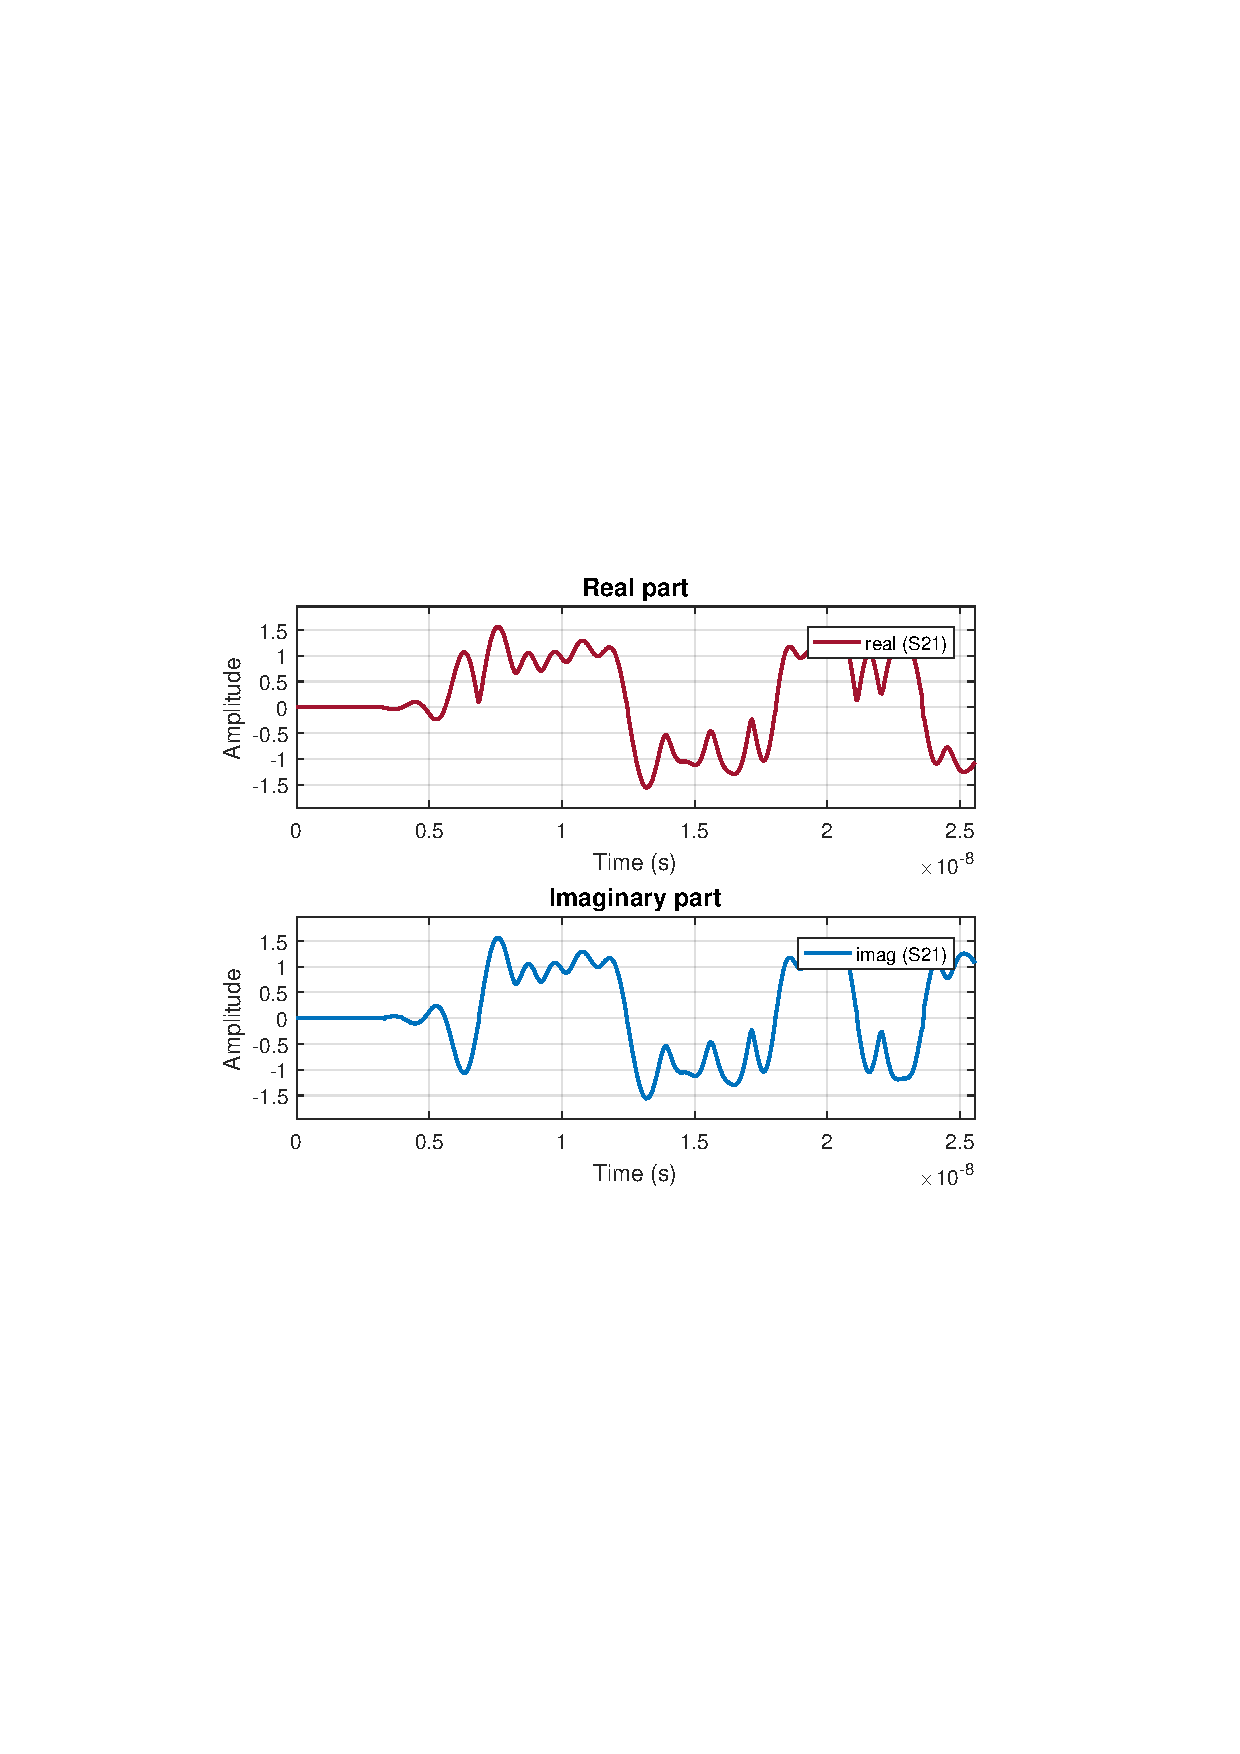
\includegraphics[width=\linewidth]{./sdf/dsp_laser_phase_compensation/figures/S24_td_v2.pdf}
  \caption{}
  \label{fig:sub1}
\end{subfigure}%
\begin{subfigure}{.5\textwidth}
  \centering
  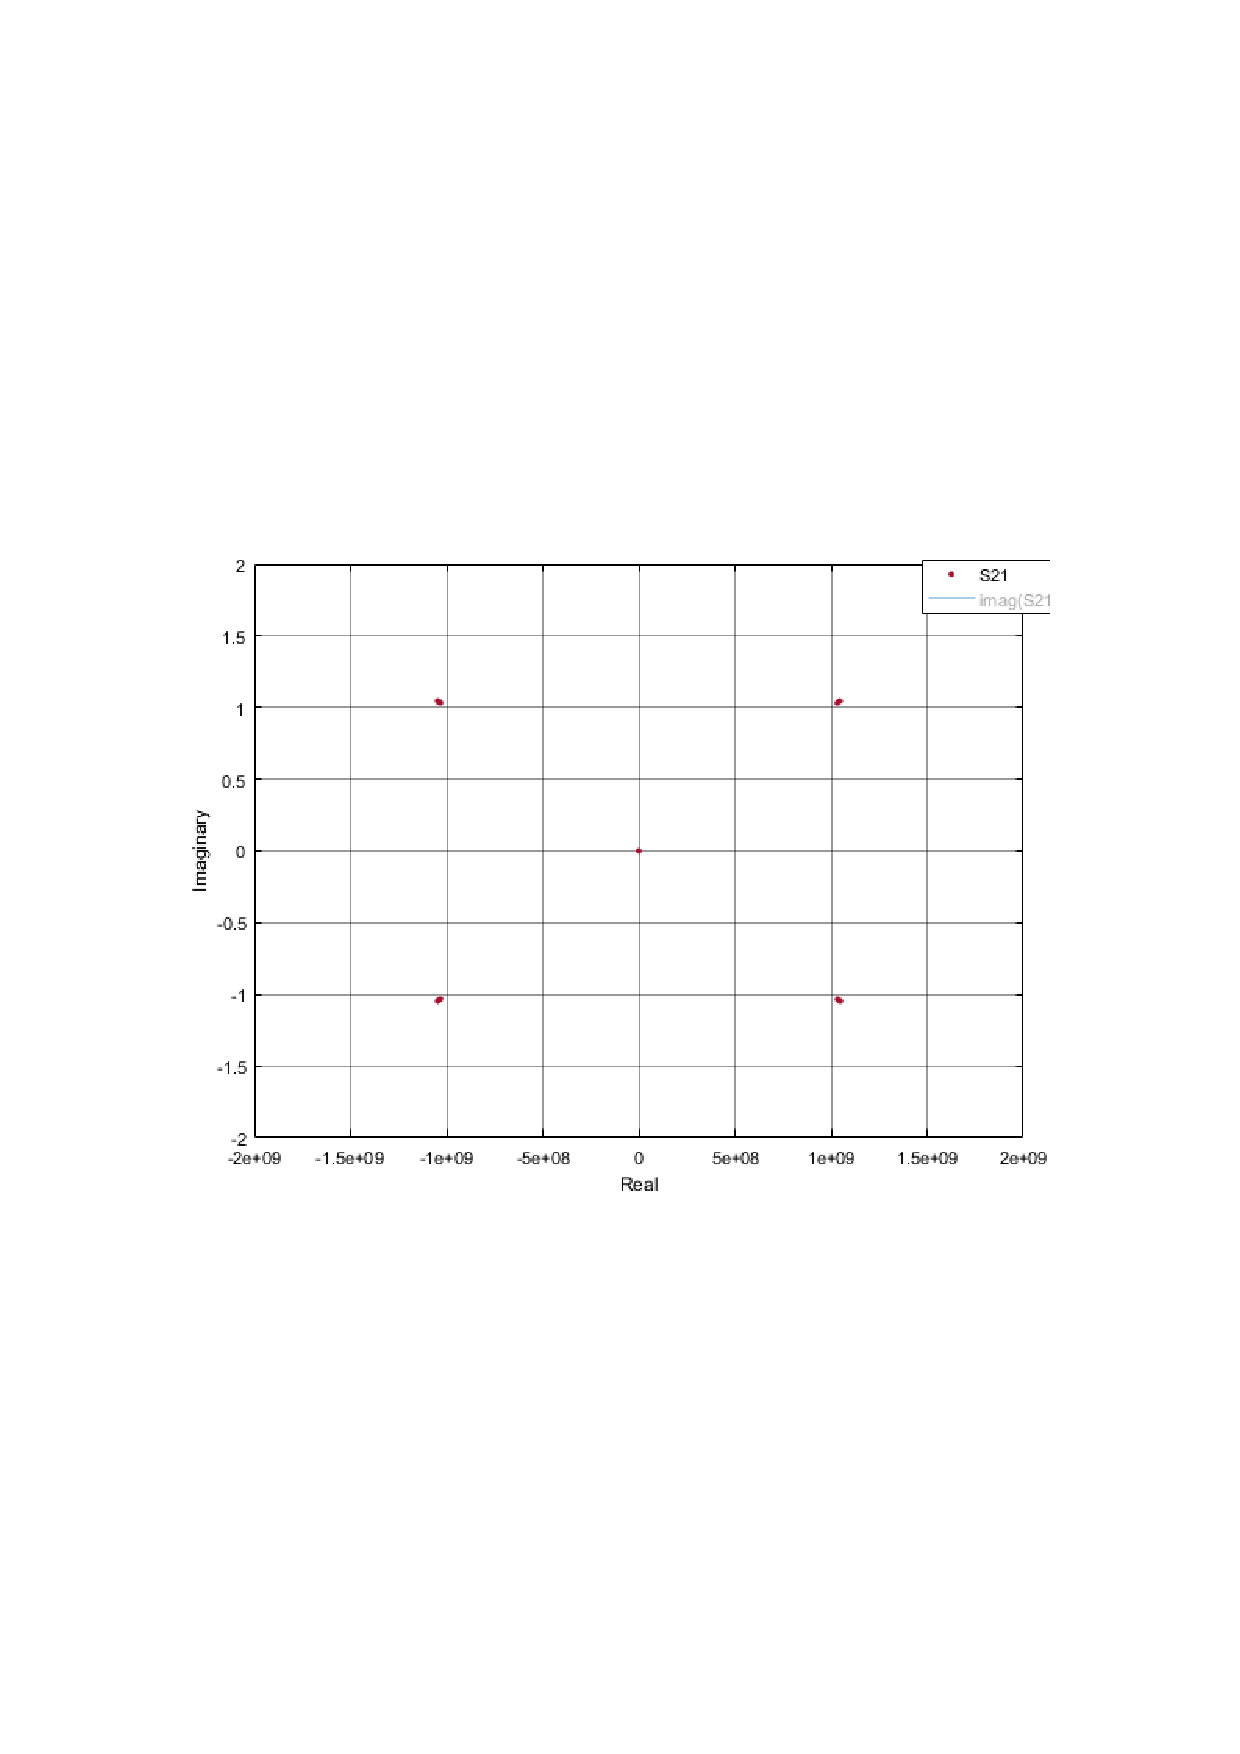
\includegraphics[width=\linewidth]{./sdf/dsp_laser_phase_compensation/figures/S24_constl_v2.pdf}
  \caption{}
  \label{fig:sub2}
\end{subfigure}
\caption{The signal after DSP block including VV algorithm for laser phase noise compensation. (a) Time-domain signal; (b)  Constellation diagram.}
\label{fig_s24}
\end{figure}

\begin{figure}[h!]
\centering
\begin{subfigure}{.5\textwidth}
  \centering
  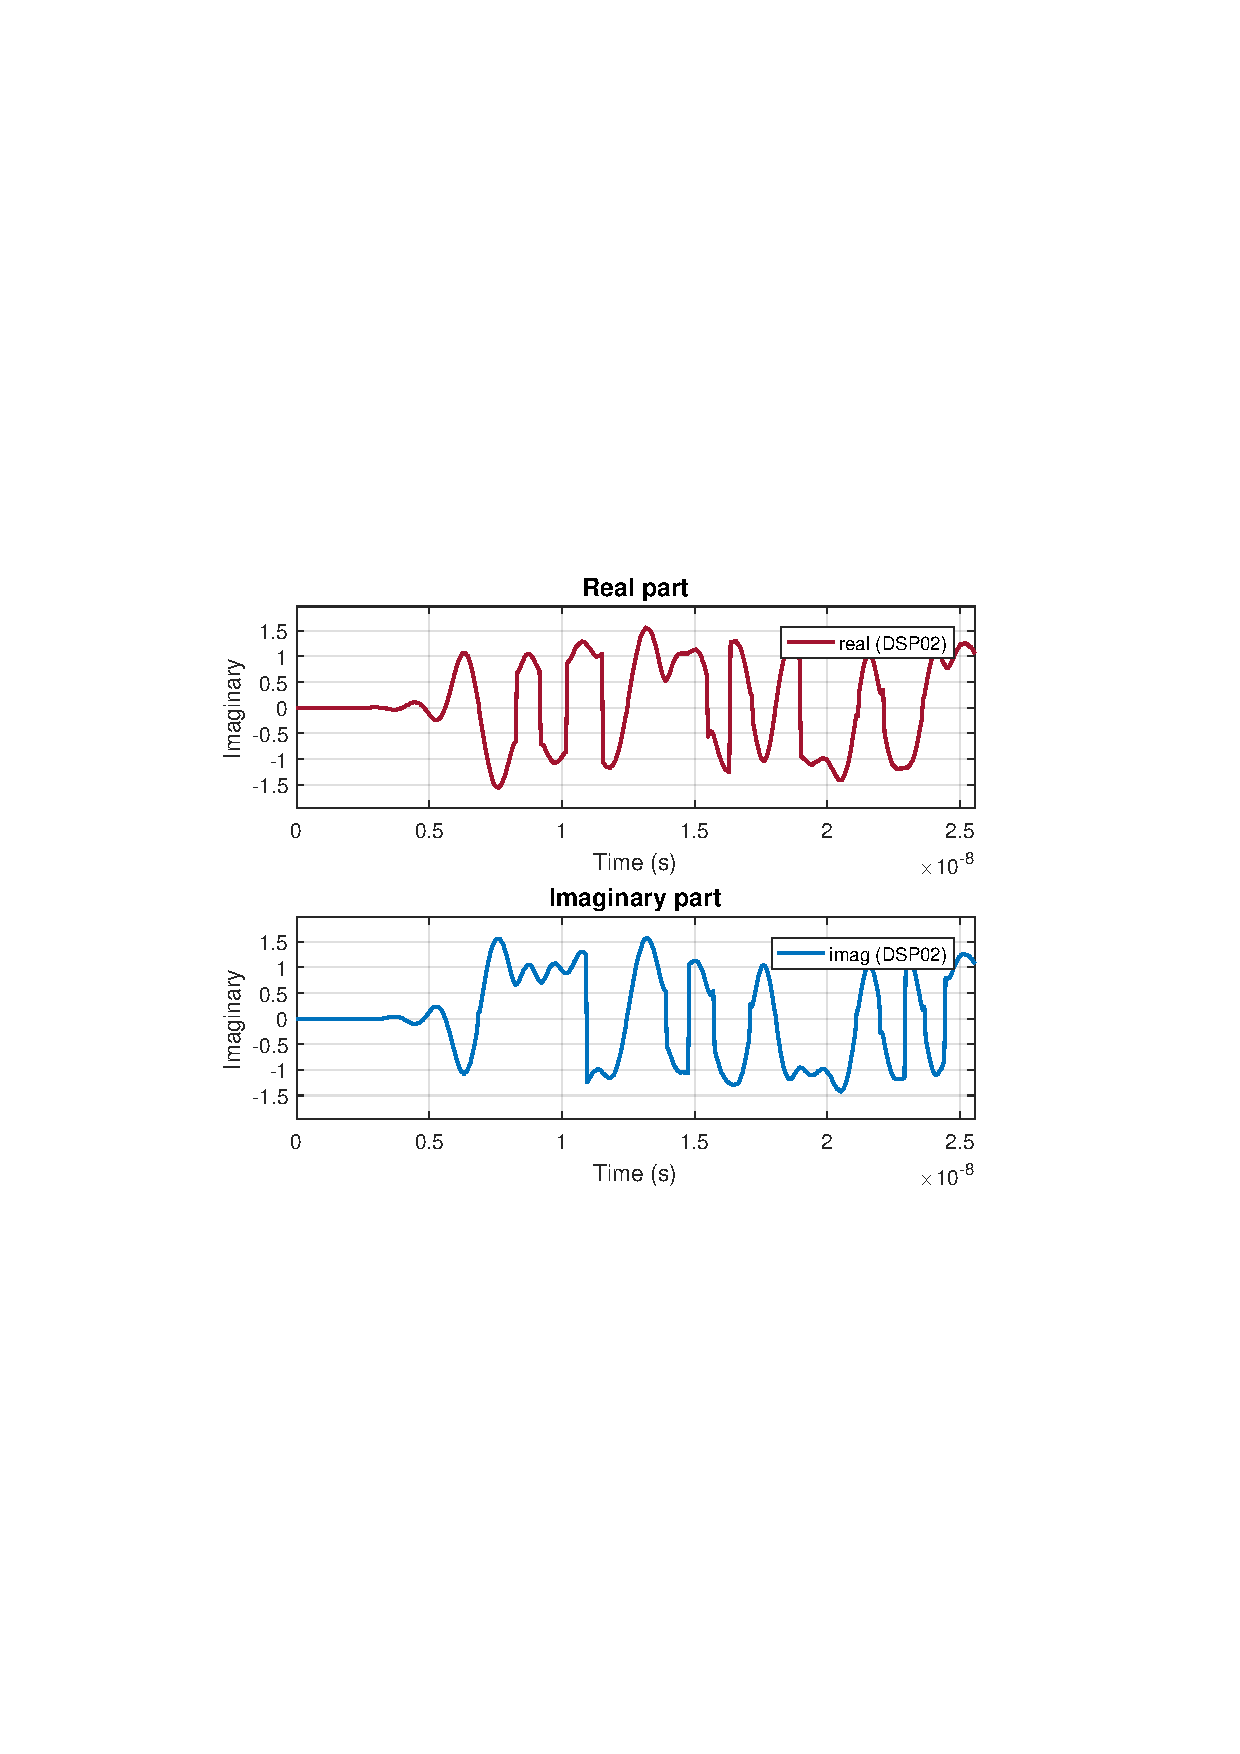
\includegraphics[width=\linewidth]{./sdf/dsp_laser_phase_compensation/figures/S24_td_bps.pdf}
  \caption{}
  \label{fig:sub1}
\end{subfigure}%
\begin{subfigure}{.5\textwidth}
  \centering
  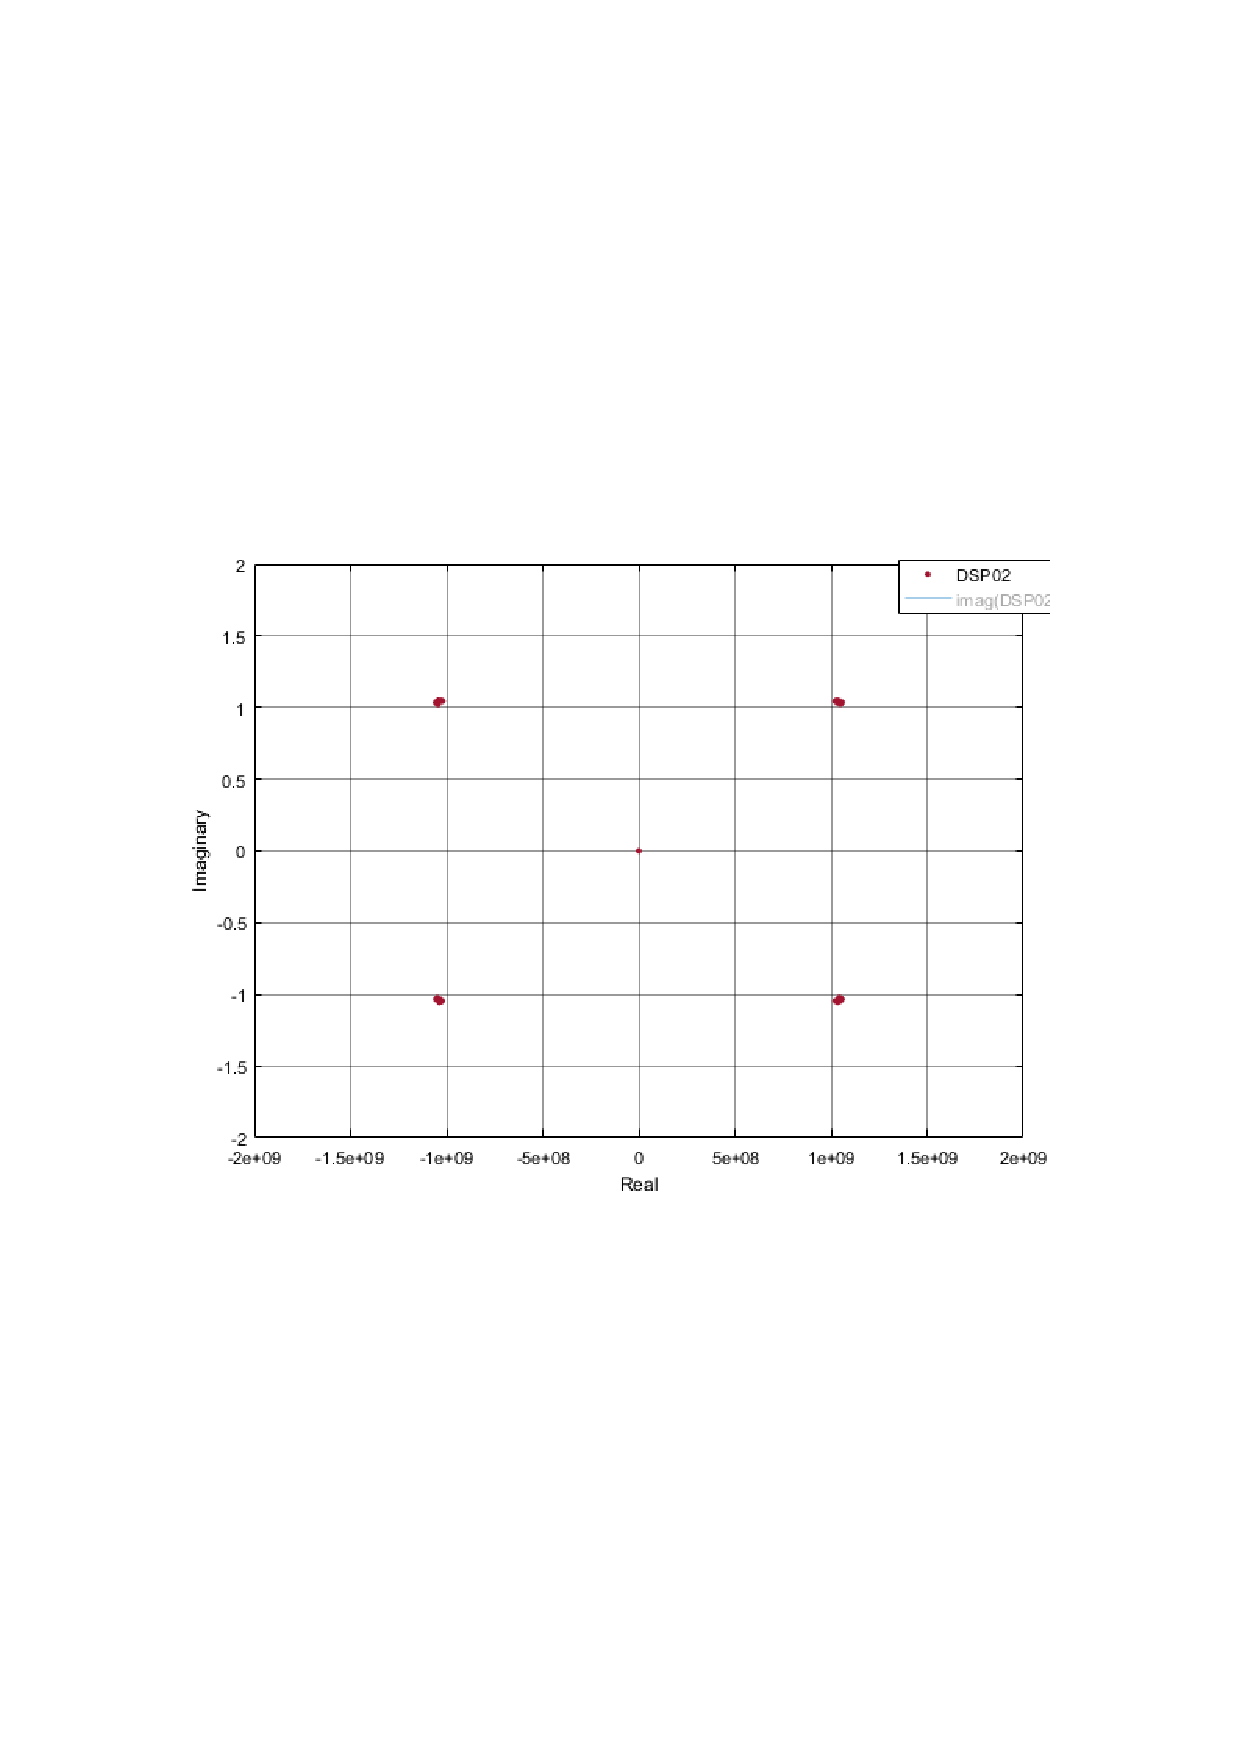
\includegraphics[width=\linewidth]{./sdf/dsp_laser_phase_compensation/figures/S24_constl_bps.pdf}
  \caption{}
  \label{fig:sub2}
\end{subfigure}
\caption{The signal after DSP block including BPS algorithm, using 64 test phases, for laser phase noise compensation. (a) Time-domain signal; (b)  Constellation diagram.}
\label{fig_s24_bps}
\end{figure}

\subsection{VHDL Implementation}

The top level implementation diagram of BPS algorithm in Very high speed integrated circuit (VHSIC) Hardware Description Language (VHDL) is shown in Figure~\ref{fig_cpeVhdlL0}. The design is based on the interconnection of several entities blocks, which performs a given function and describe the interface signals into and out of the design unit.
The input signal to the top level entity block $\textit{CPE\_BPS}$ is provided by testbench, which defines the stimuli for the simulation of unit under test (UUT). The input signal is loaded from an external file, converted into $\textit{std\_logic\_vector}$ type and then sent to the UUT. The output of UUT of $\textit{std\_logic\_vector}$ type is converted integer type and then save into external file.


\subsubsection{Top Level Implementation of BPS Entity Block}

In $\textit{CPE\_BPS}$ block, the input signal is firstly delayed one clock cycle to be synchronized with the output of $\textit{2P-ROM-0}$, where the exponential of test phases are saved. The output of $\textit{2P-ROM-0}$ and the delayed input signal correspond to the input of $\textit{Distance Calculation}$ block, where the distance to the closest constellation points in the original constellation is calculated. The VHDL implementation diagram of $\textit{Distance Calculation}$ block is presented in the Figure~\ref{fig_DCVhdlL1} and the detail is presented later. The outputs of $\textit{Distance Calculation}$ correspond to two array of $\textit{std\_logic\_vector}$ which can be interpreted as matrixes N by M, where N is the number of test phase and M is the number of parallel processed sample. One output holds the values of distance calculation and the other output hold the ROM address for the corresponding decision from $Decision Circuit$ of square distance calculation block, Figure~\ref{fig_SDVhdlL2}.
The two N$\times$M matrixes outputs of $\textit{Distance Calculation}$ are converted to M$\times$N matrixes using $\textit{Array2Array}$ entity block. Then, the output holding the values of distance calculation correspond to the input of $\textit{MinArray}$ entity block, where the minimum distance for each $M$ input samples are determined. For complexity reduction purpose, the output of $\textit{MinArray}$ is a $\textit{std\_logic\_vector}$ holding $M$ indexes of minimum distance values. In parallel to the minimum distance search, the matrix holding the ROM addresses is delayed to be synchronized with the output of $\textit{MinArray}$, which are then the input of $\textit{ROM Adress Selection}$ entity block. Based on the output of $\textit{MinArray}$, the block $\textit{ROM Adress Selection}$ selects the addresses of decoded output symbol from IQ signal ROM. The $M$ addresses obtained from $\textit{ROM Adress Selection}$ are used to select the decoded output symbol from IQ signal ROM.


\begin{figure}[h!]
    \centering
    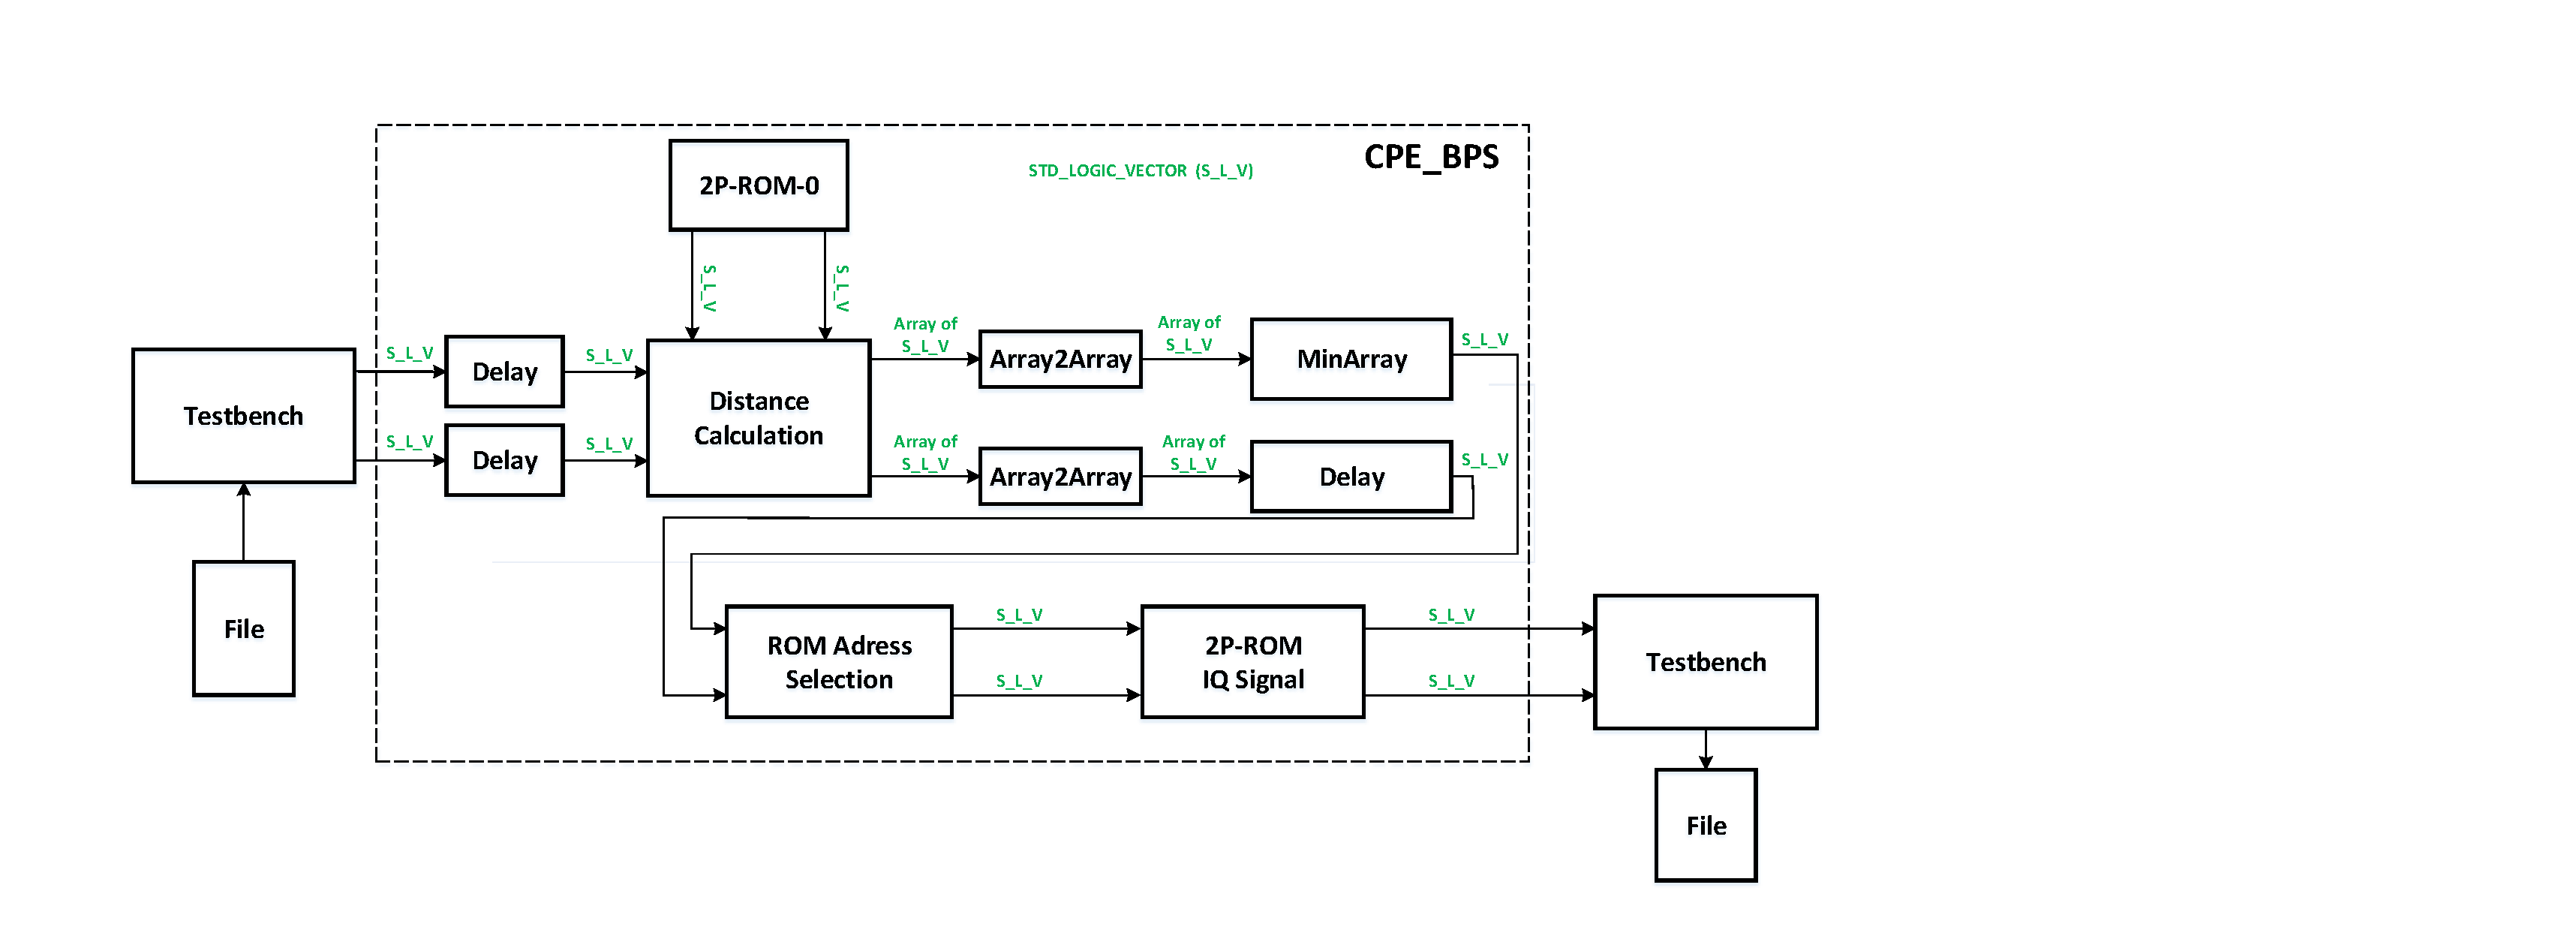
\includegraphics[width=15cm]{./sdf/dsp_laser_phase_compensation/figures/cpe_bps.pdf}
    \caption{Top level entity block for VHDL implementation of BPS.}
    \label{fig_cpeVhdlL0}
\end{figure}

\subsubsection{Implementation of Distance Calculation Entity Block}

The $\textit{Distance Calculation}$ entity block is interfaced by four inputs and two outputs of $\textit{std\_logic\_vector}$ type. The inputs correspond to the real and imaginary of input samples and test phase. The outputs are the corresponding distance between the rotated input sample to the closest constellation points and the ROM address of corresponding symbol decision.
$\textit{Distance Calculation}$ entity block is composed by the interconnection of 3 entity blocks. Firstly, the square distance are calculated and the ROM address of symbol decision are determined by $\textit{Distance Calculation}$ entity block. The consecutive calculated distances are buffered using $\textit{Buffer}$ entity block, which is then the input of $\textit{Average}$ entity block for the average calculation. In parallel, the ROM address output is delayed to be synchronized with the output of $\textit{Average}$ entity block.

\begin{figure}[h!]
    \centering
    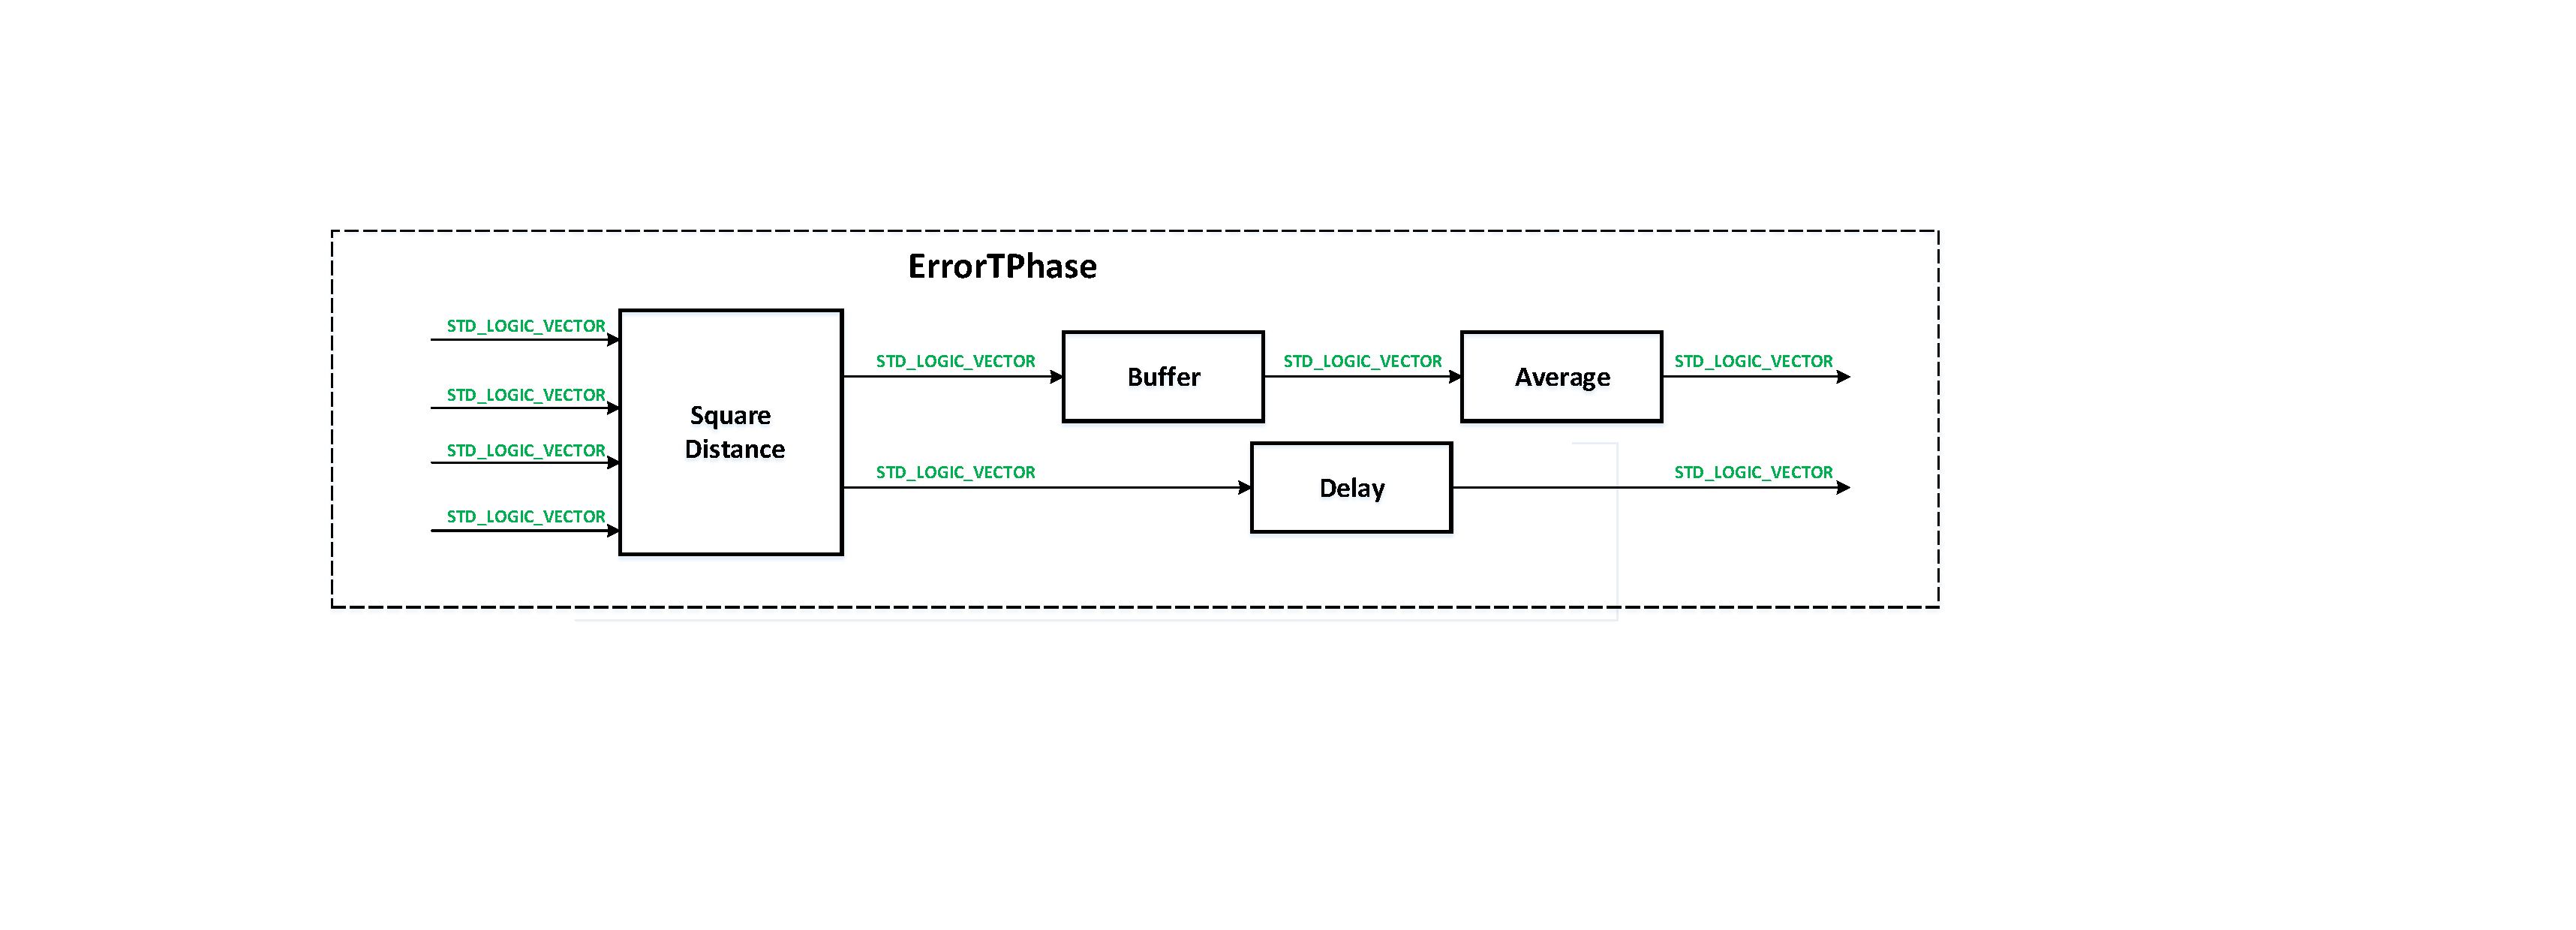
\includegraphics[width=12cm]{./sdf/dsp_laser_phase_compensation/figures/errorTphase.pdf}
    \caption{VHDL implementation of sub-block of CPE for the distance calculation between the signal and $N$ test phases.}
    \label{fig_DCVhdlL1}
\end{figure}


\subsubsection{Implementation of Square Distance Calculation Entity Block}

The $\textit{Square Distance Calculation}$ entity block has the same inputs and outputs as $\textit{Distance Calculation}$ entity block. The first operation correspond to the complex multiplication between the input sample and the test phase. The result is then fed to the $\textit{Decision Circuit}$ entity block, where the symbol decision is performed. The output of $\textit{Decision Circuit}$ is the ROM address of corresponding decoded symbol. The ROM outputs and the delay version of complex multiplication are then fed to the $\textit{Complex Subtration}$ entity block followed by its absolute value calculation. The output of $\textit{Absolute Value}$ entity block is then registered, which is the output of $\textit{Square Distance Calculation}$ entity block in parallel with the delayed ROM address of decoded symbol.


\begin{figure}[h!]
    \centering
    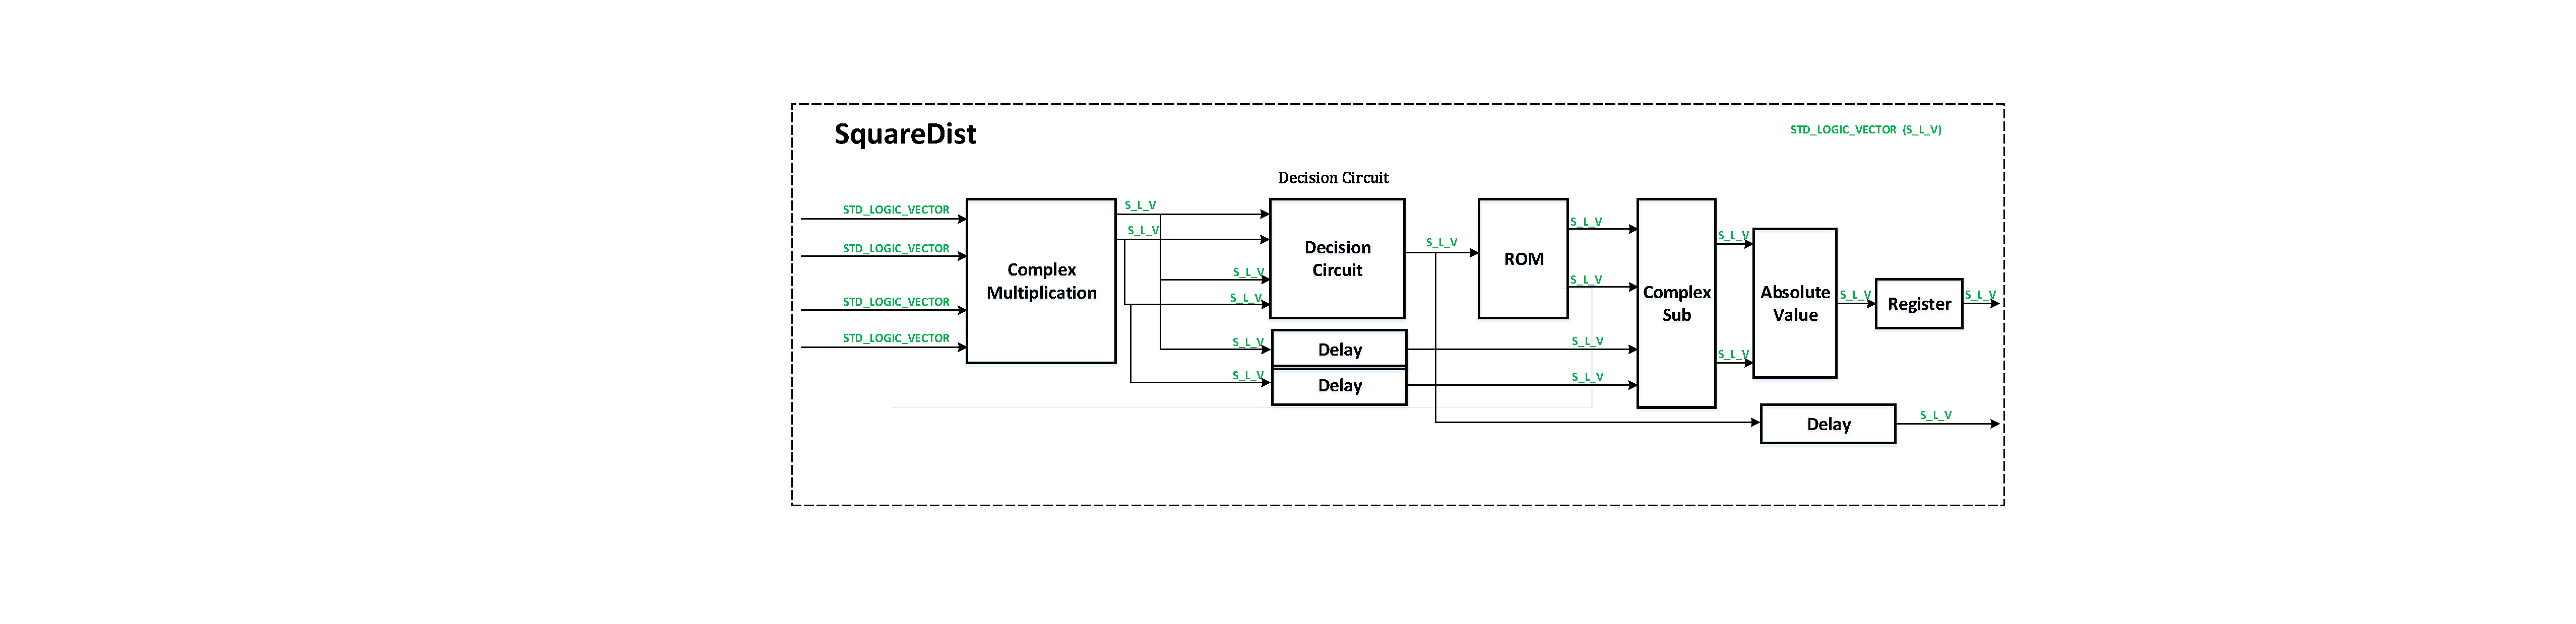
\includegraphics[width=15cm]{./sdf/dsp_laser_phase_compensation/figures/squareDist.pdf}
    \caption{VHDL implementation of sub-block of CPE for the square distance calculation between the signal and one test phase.}
    \label{fig_SDVhdlL2}
\end{figure}

%  COLOCAR ESTAS REFERÊNCIAS NUM FICHEIRO BIB
%
%	\bibitem{latexcompanion}
%	Munier, E. Alpman, T. Eriksson, A. Svensson, and H. Zirath.
%	\textit{Estimation of phase noise for QPSK modulation over AWGN channels}.
%	in Proc. GigaHertz 2003 Symp., Sweden, Nov. 4-5, 2003.
%	
%	\bibitem{latexcompanion}
%	T. Pfau, S. Hoffmann, and R. No\`{e}.
%	\textit{Estimation of phase noise for QPSK modulation over AWGN channels}.
%    J. Lightw. Technol., vol. 27, no. 8, pp. 989-999, Apr. 15, 2009.
%


% bibliographic references for the section ----------------------------
\clearpage
\printbibliography[heading=subbibliography]
\end{refsection}
\addcontentsline{toc}{subsection}{Bibliography}
\cleardoublepage
% --------------------------------------------------------------------- 